\section{Numerical Experiments/ Results}\label{chap:experiments}
\iffalse
check angle preservation (e.g., via dot products on mapped vectors) and scale factors ($det(D\Phi) > 0$, $|\frac{\del\Phi}{\del z}|$ constant in theory).
- Test suite: Use known exact mappings (e.g., disk to square via Schwarz-Christoffel) for error metrics (L2 norm on boundary points).
- Metrics: Runtime for N points, mesh quality post-mapping (e.g., min/max angles in triangles, shape regularity ratio).
- Real-world applicability: Apply to a sample FEM problem (e.g., Poisson equation on $\Omega$) and compare accuracy/speed vs. uniform mesh.
- Robustness: Vary boundary complexity (smooth vs. corners), noise in Fourier coeffs, mesh resolutions.
- Debugging: Use assertions for bijectivity (e.g., check injectivity numerically)
- Error handling - what happens with degenerate inputs?
\fi
Remark. Note that in order to avoid confusion with the word 'method' in programming, we have chosen to use the german word 'Verfahren' to refer to the two different approaches described in Wegmann's paper.
\bigskip
Experiments conducted with the two Verfahren of the solver have confirmed the results Wegmann got with regard to convergence: Verfahren 2 typically converges faster. However, Wegmann claims that Verfahren 1 typically yields more accurate results, which we have not been able to reproduce. 
We present some illustrations of our results in this chapter.
In order to be able to measure the accuracy of the result computed by the solver, we relied on some explicitly known conformal maps, which are provided by Gaier in his book \cite[Anhang 5, p. 264]{Gaier1964}. 
The measure of accuracy in the below tables is calculated as the $L^2$-norm of the difference of the functions at the respective discretisation points.

\newpage
%%%%%%%%%%%% ECCENTRIC CIRCLE %%%%%%%%%%%%%%%%%%%
\begin{figure}[H]
    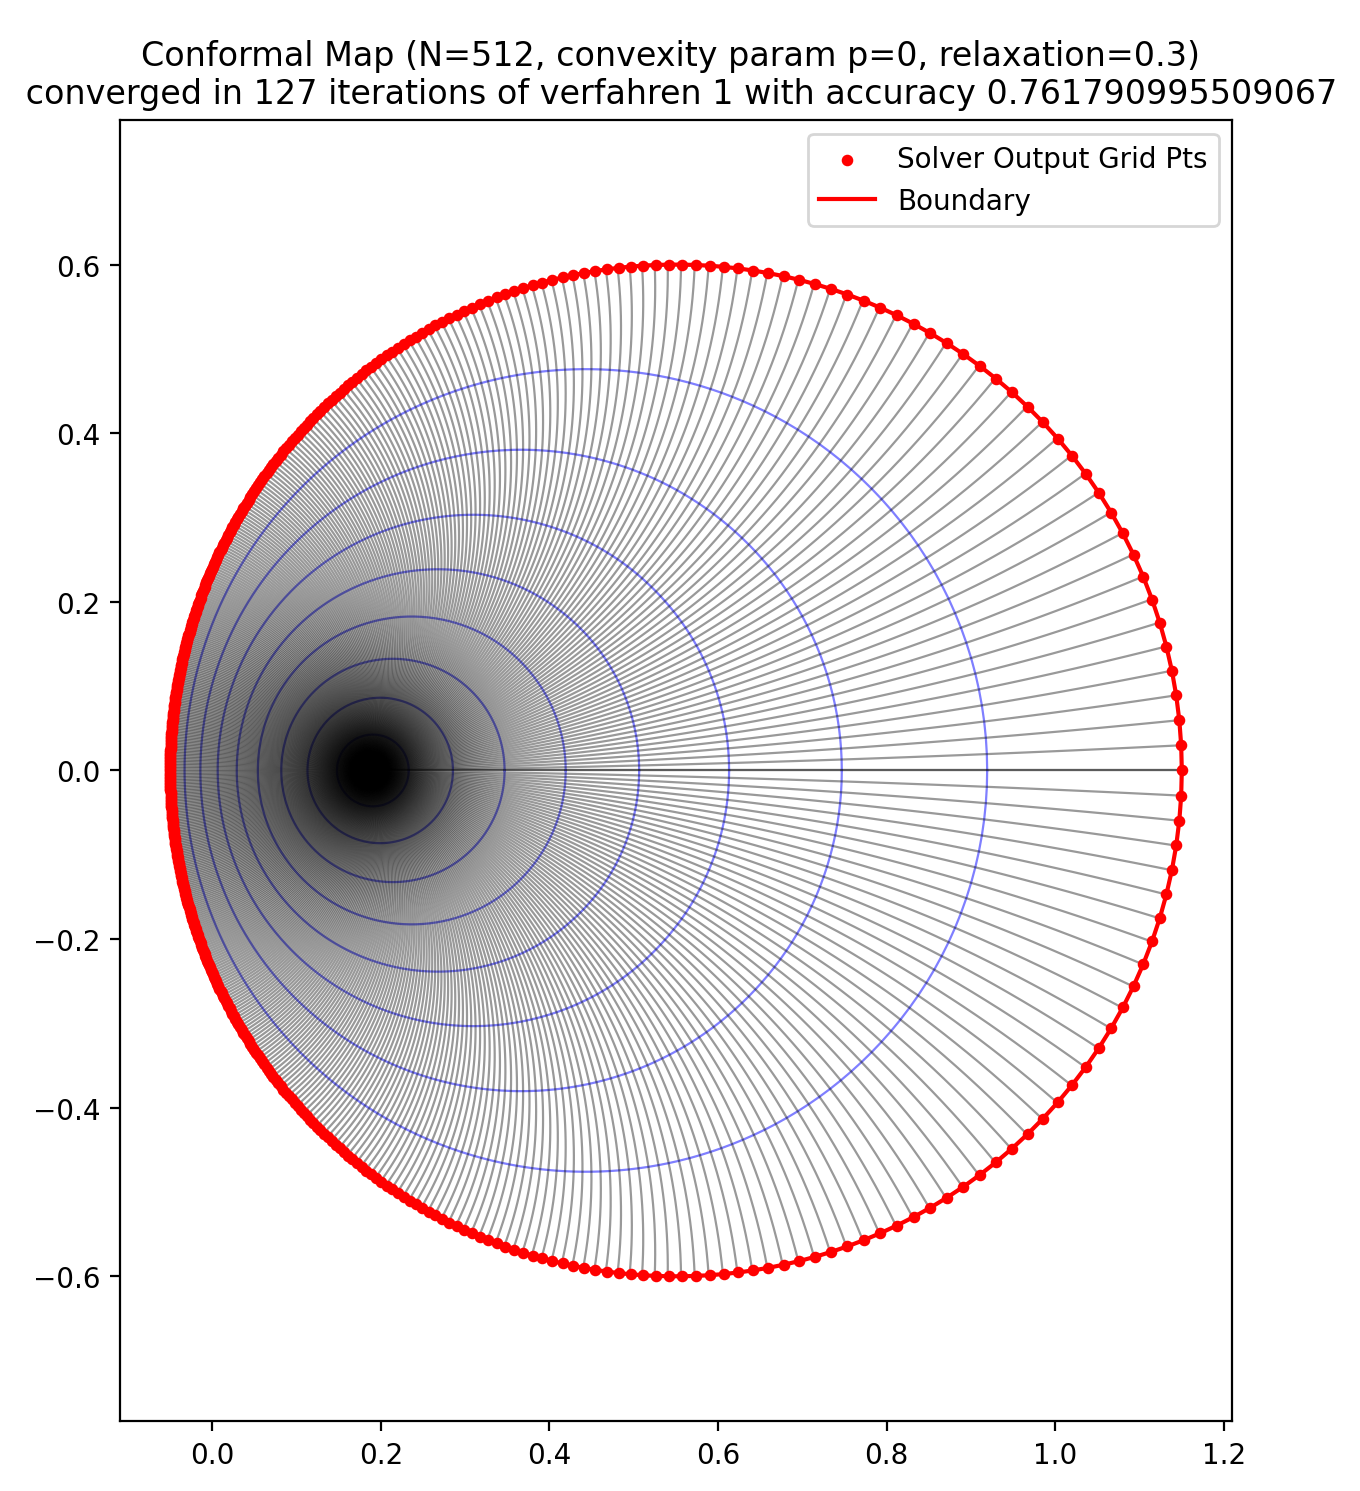
\includegraphics[width=0.5\textwidth]{img/eccentric_v1_rel3.png}
    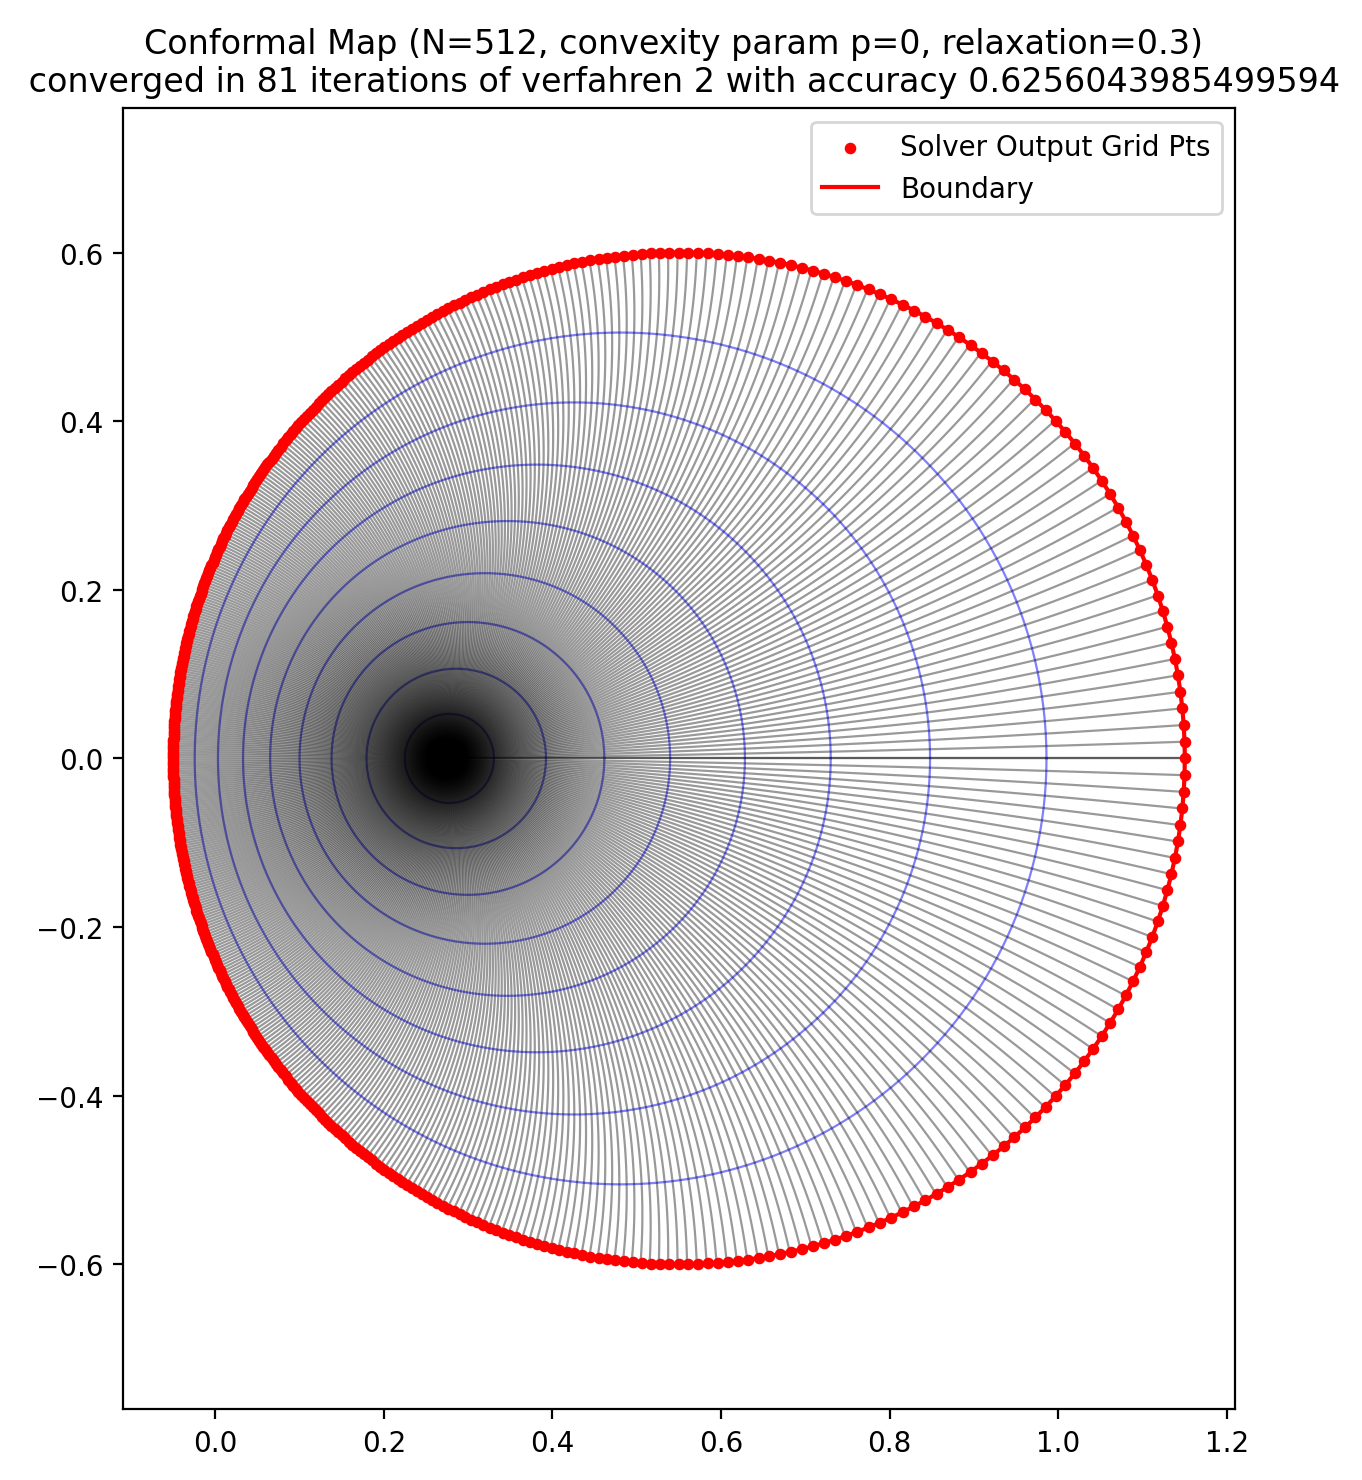
\includegraphics[width=0.5\textwidth]{img/eccentric_v2_rel3.png}
    \caption{Gaier's eccentric circle. \cite[Anhang 5, p. 264]{Gaier1964}}
\end{figure}

\begin{table}[H] %\centering
    \caption{Eccentric circle discretized at $N = 512$ points.}
    \begin{tabular}{|p{0.2\textwidth}|p{0.35\textwidth}|p{0.35\textwidth}|}
        \hline
        Verfahren & 1 & 2 \\
        \hline
        Accuracy & 0.761790995509067 & 0.6256043985499594 \\
        \hline
        Iteration \# & \multicolumn{2}{c}{Norm of correction/ update step $\lVert U_{k} \rVert$} \\
        0 & 720.3882650364529 & 720.3882650364529 \\
        1 & 240.96871847609182 & 345.28799456238954 \\
        2 & 123.03673246529644 & 181.9463636411823 \\
        3 & 74.77256117097478 & 113.31865680003762 \\
        4 & 49.23654870031479 & 75.15166708336353 \\
        5 & 34.0021274191191 & 51.27741887350757 \\
        6 & 24.257897110960663 & 35.466301329451 \\
        7 & 17.731997779526324 & 24.69504948431332 \\
        8 & 13.212311049497963 & 17.252206390803625 \\
        9 & 9.99841060567796 & 12.072094322857915 \\
        10 & 7.662812612112827 & 8.453676136529895 \\
        \dots & \dots & \dots \\
        81 & 1.7080984717844722e-06 & 8.53657643311748e-11 \\
        \dots & \dots &  \\
        127 & 9.666774826434523e-11 & \\
        \hline
    \end{tabular}
\end{table}

\newpage
%%%%%%%%%%%% INVERTED ELLIPSE p=0.6 %%%%%%%%%%%%%%%%%%%
\begin{figure}[H]
    \caption{Gaier's inverted ellipse, which is also Wegmann's flagship example. Convexity parameter: $p=0.6$ \cite[Anhang 5]{Gaier1964} \cite[§6]{Wegmann1978_newtonverfahren}}
    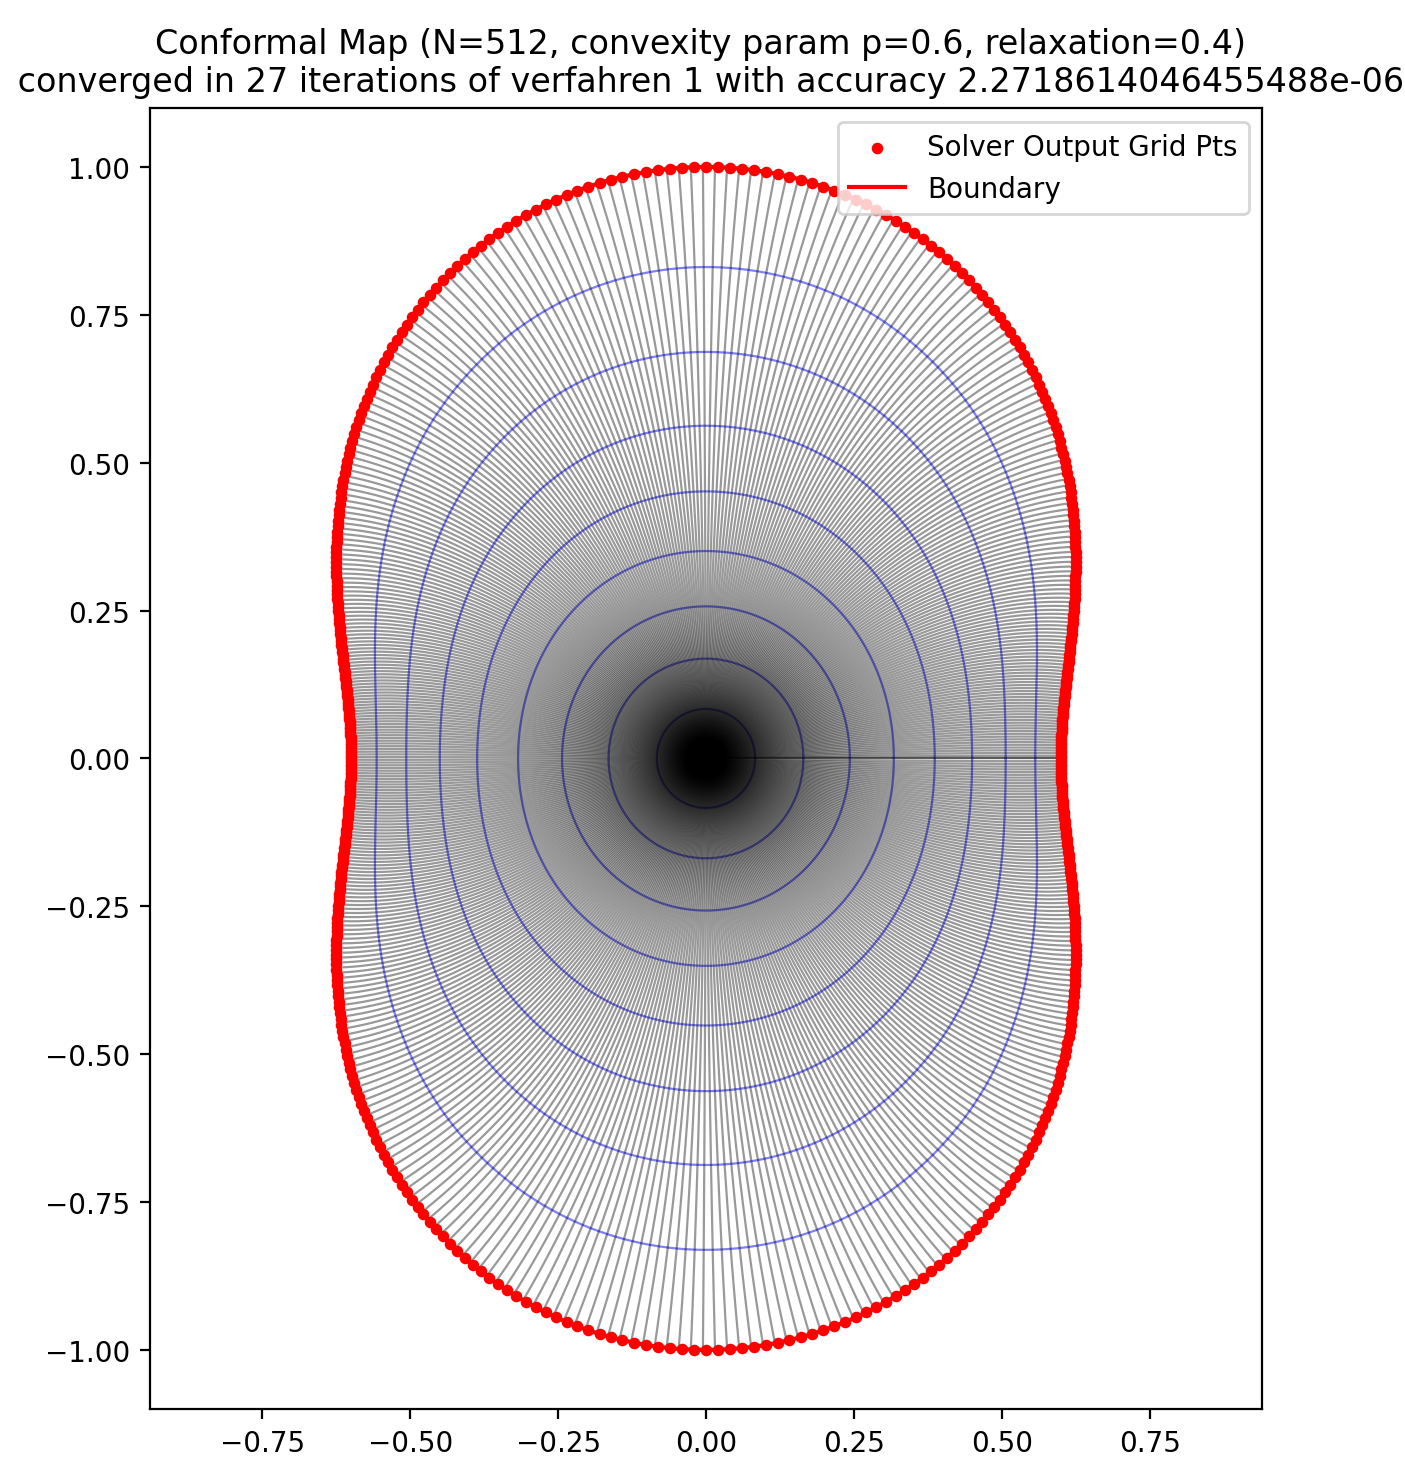
\includegraphics[width=0.5\textwidth]{img/invellip_v1_p6_rel4.png}
    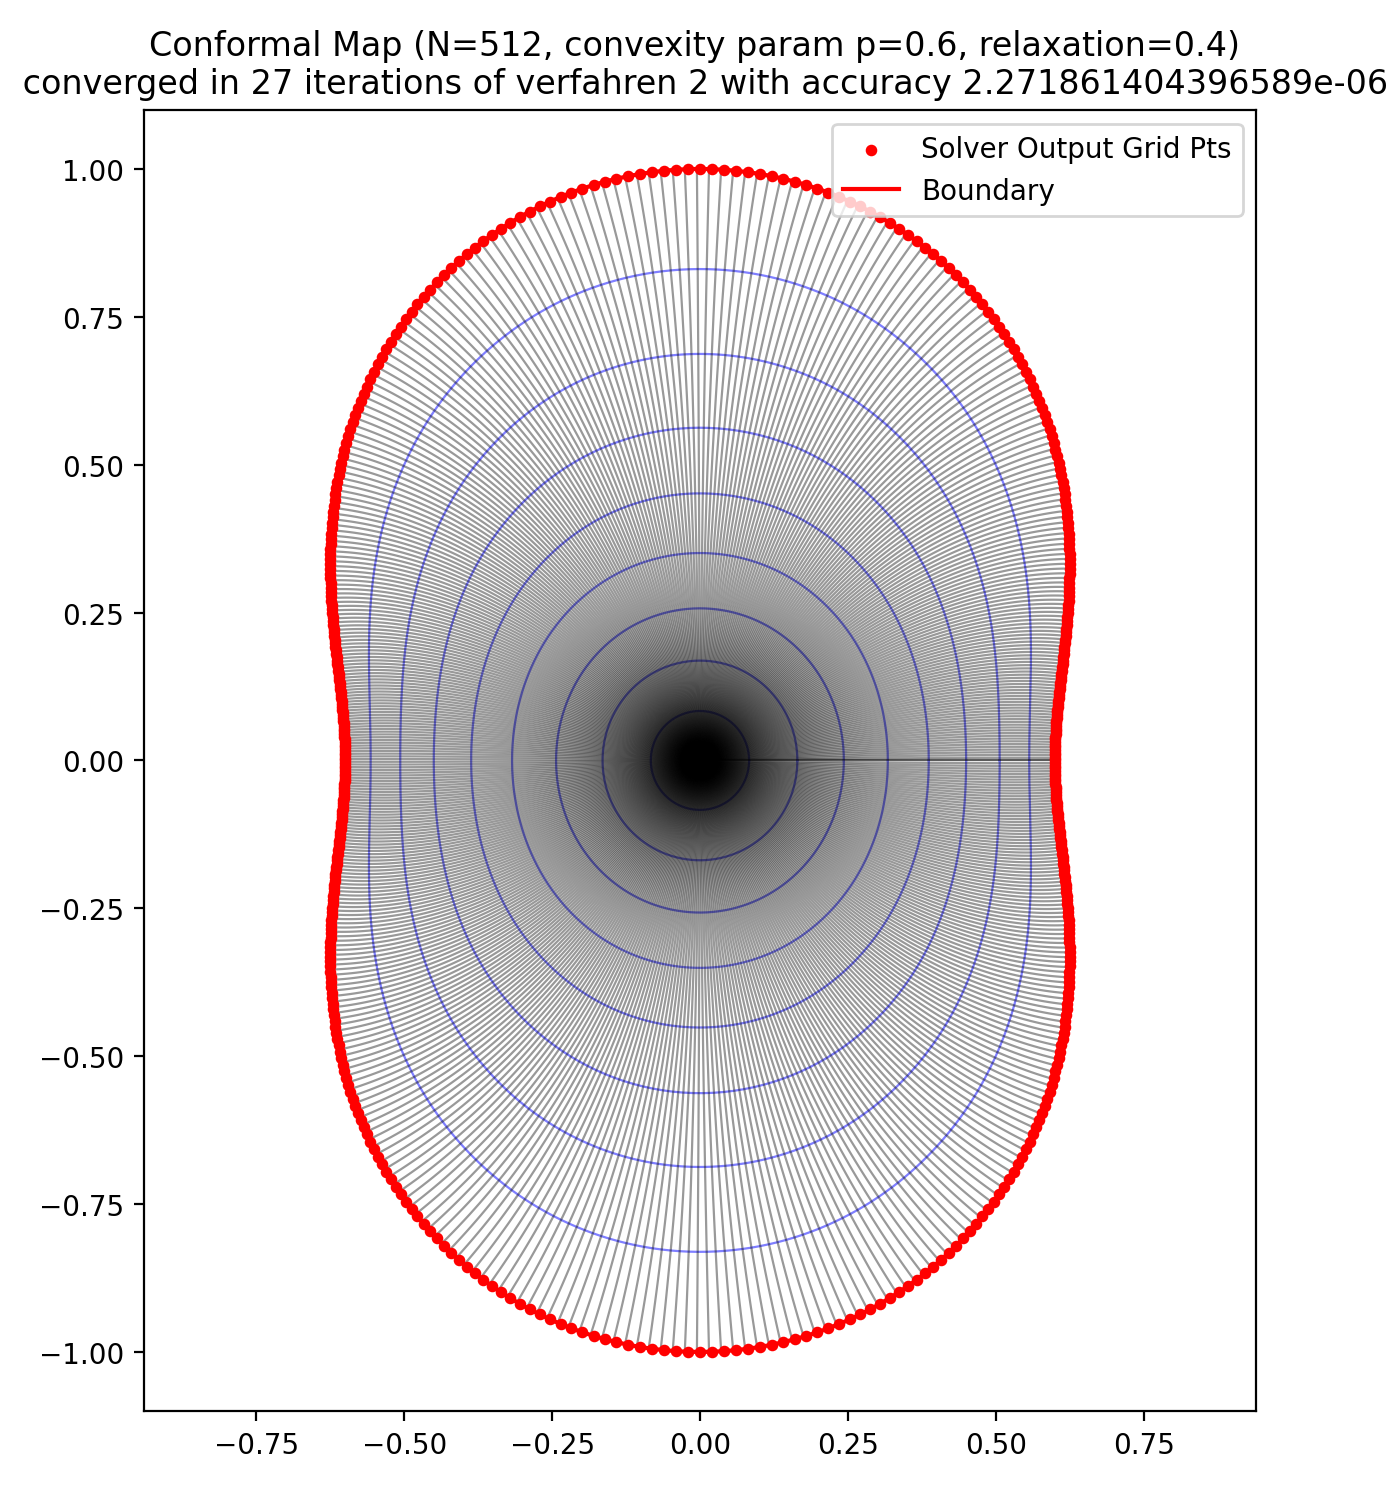
\includegraphics[width=0.5\textwidth]{img/invellip_v2_p6_r4.png}
\end{figure}

\begin{table}[H] \centering
    \caption{Inverted ellipse discretized at $N = 512$ points, with convexity parameter $p = 0.6$.}
    \begin{tabular}{|p{0.2\textwidth}|p{0.35\textwidth}|p{0.35\textwidth}|}
        \hline
        Verfahren & 1 & 2 \\
        \hline
        Accuracy & 2.2718614046455488e-06 & 2.271861404396589e-06 \\
        \hline
        Iteration \# & \multicolumn{2}{c|}{Norm of correction/ update step $\lVert U_{k} \rVert$} \\
        \hline
        0 & 88.63480431858018 & 88.63480431858018 \\
        1 & 54.90539548249176 & 54.90539548249178 \\
        2 & 33.61316776554185 & 33.61316776554185 \\
        3 & 20.41971454542174 & 20.419714545421737 \\
        4 & 12.344745234840195 & 12.344745234840188 \\
        5 & 7.440777181665198 & 7.440777181665202 \\
        6 & 4.476783261513716 & 4.476783261513759 \\
        7 & 2.690525881801778 & 2.6905258818017637 \\
        8 & 1.6159243413944206 & 1.6159243413944353 \\
        9 & 0.9701347833233221 & 0.970134783323305 \\
        10 & 0.5822899509291396 & 0.5822899509291886 \\
        \dots & \dots & \dots \\
        27 & 9.861536502951661e-05 & 9.861536505303449e-05 \\
        \hline
    \end{tabular}
\end{table}


%%%%%%%%%%%% INVERTED ELLIPSE p = 0.4 %%%%%%%%%%%%%%%%%%%
    \begin{figure}[H]
    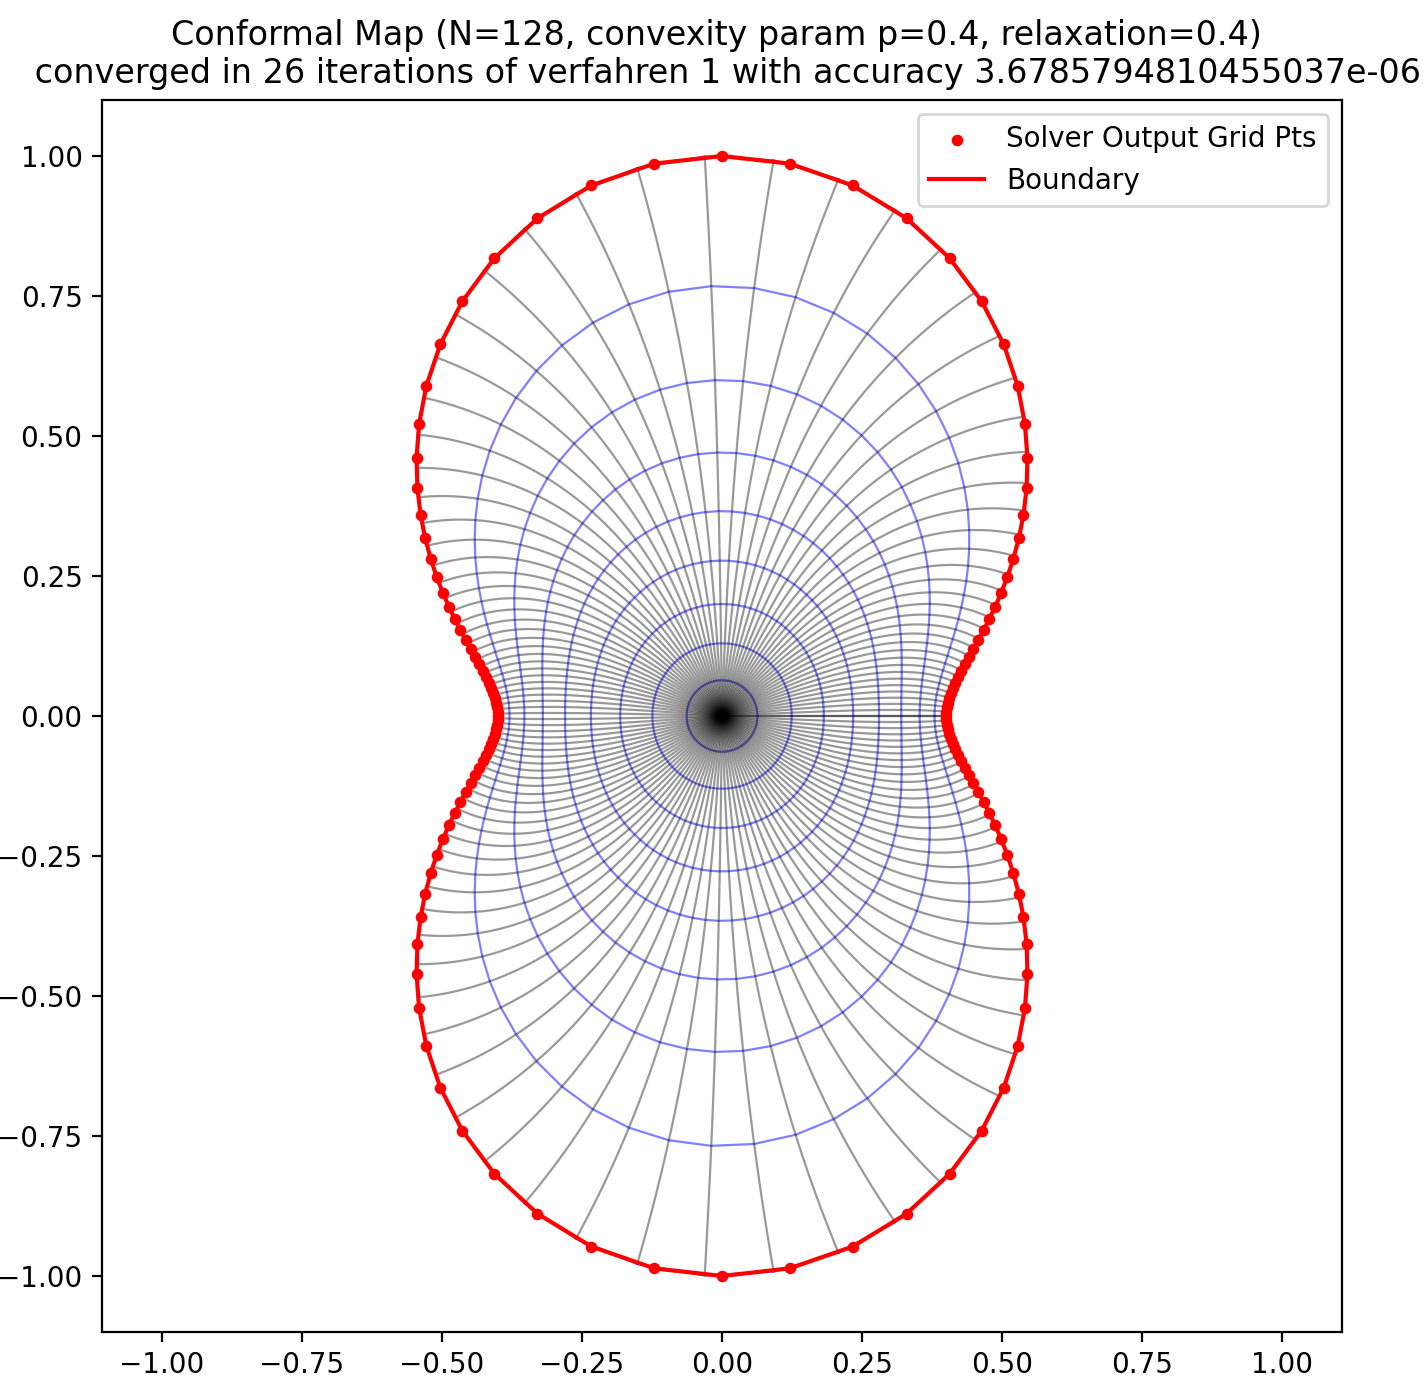
\includegraphics[width=0.5\textwidth]{img/invellip_v1_p4_r4.png}
    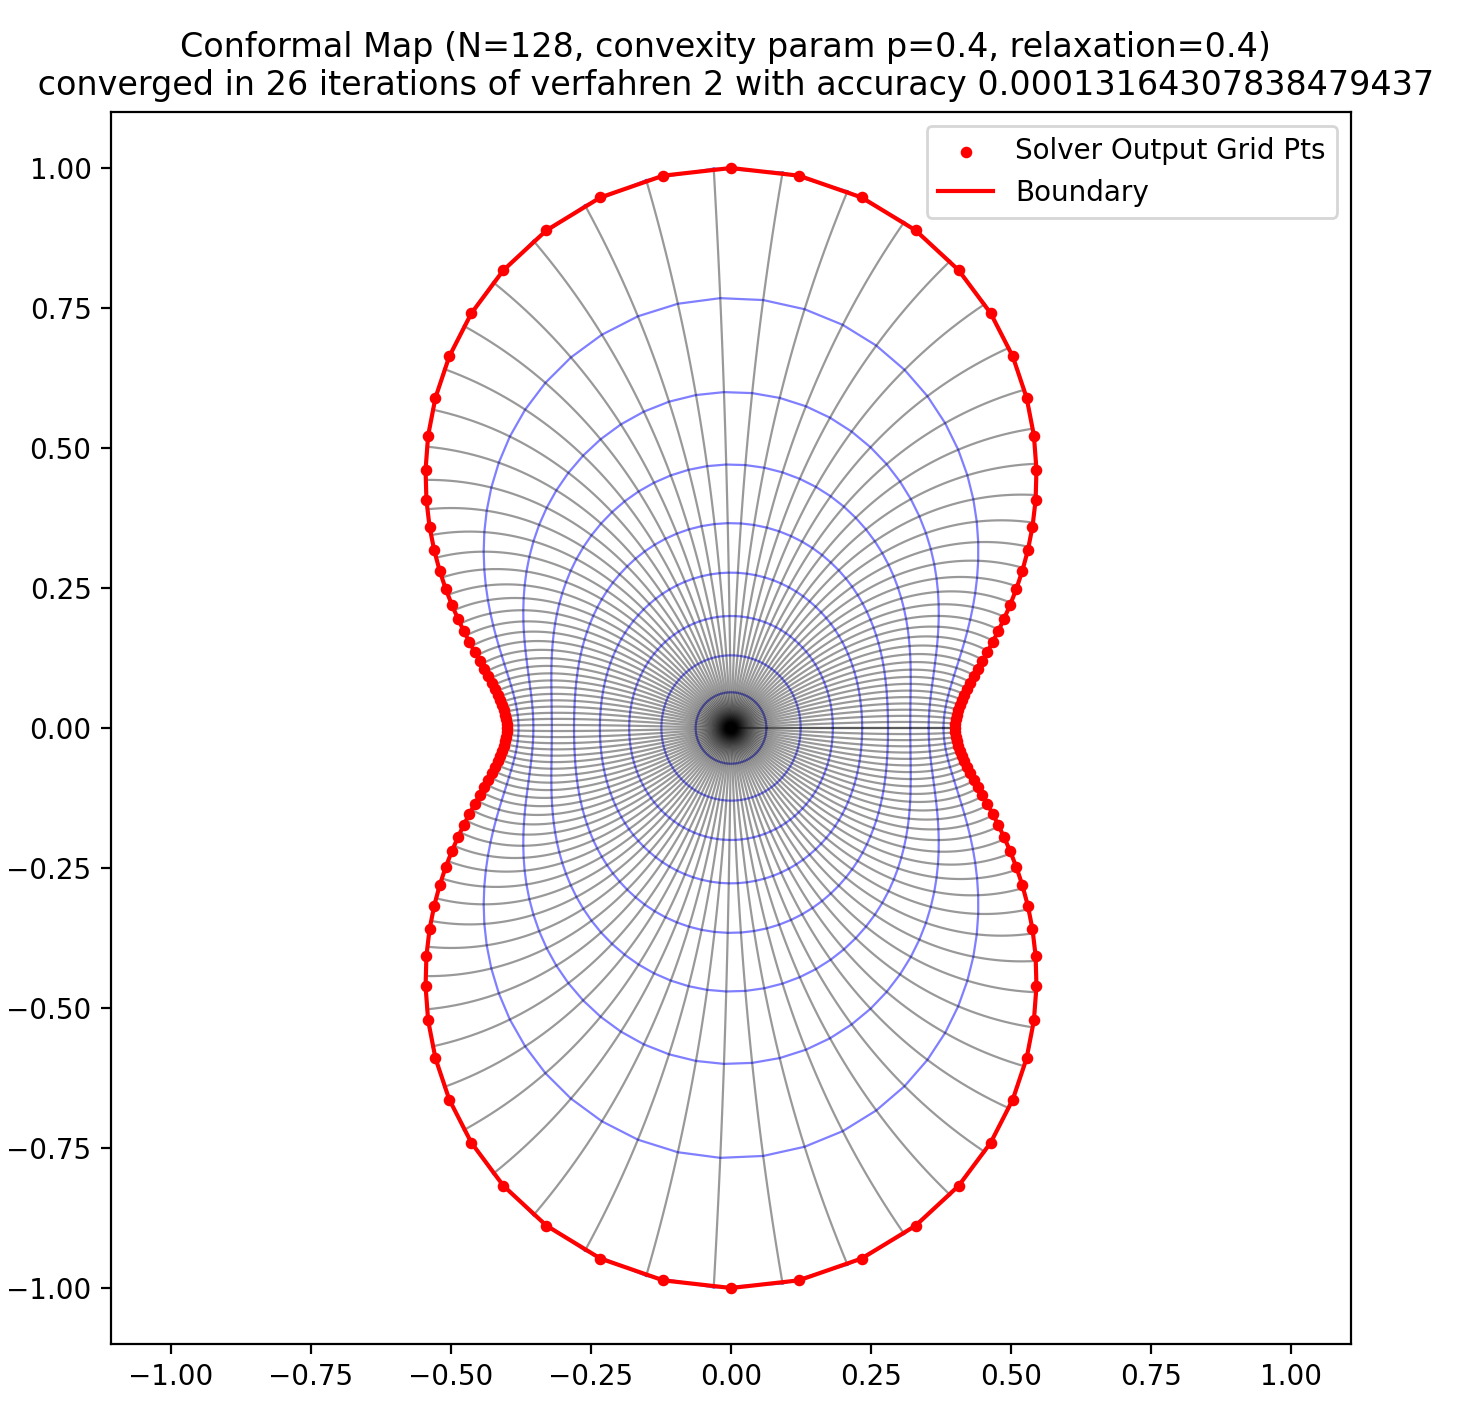
\includegraphics[width=0.5\textwidth]{img/invellip_v2_p4_r4.png}
    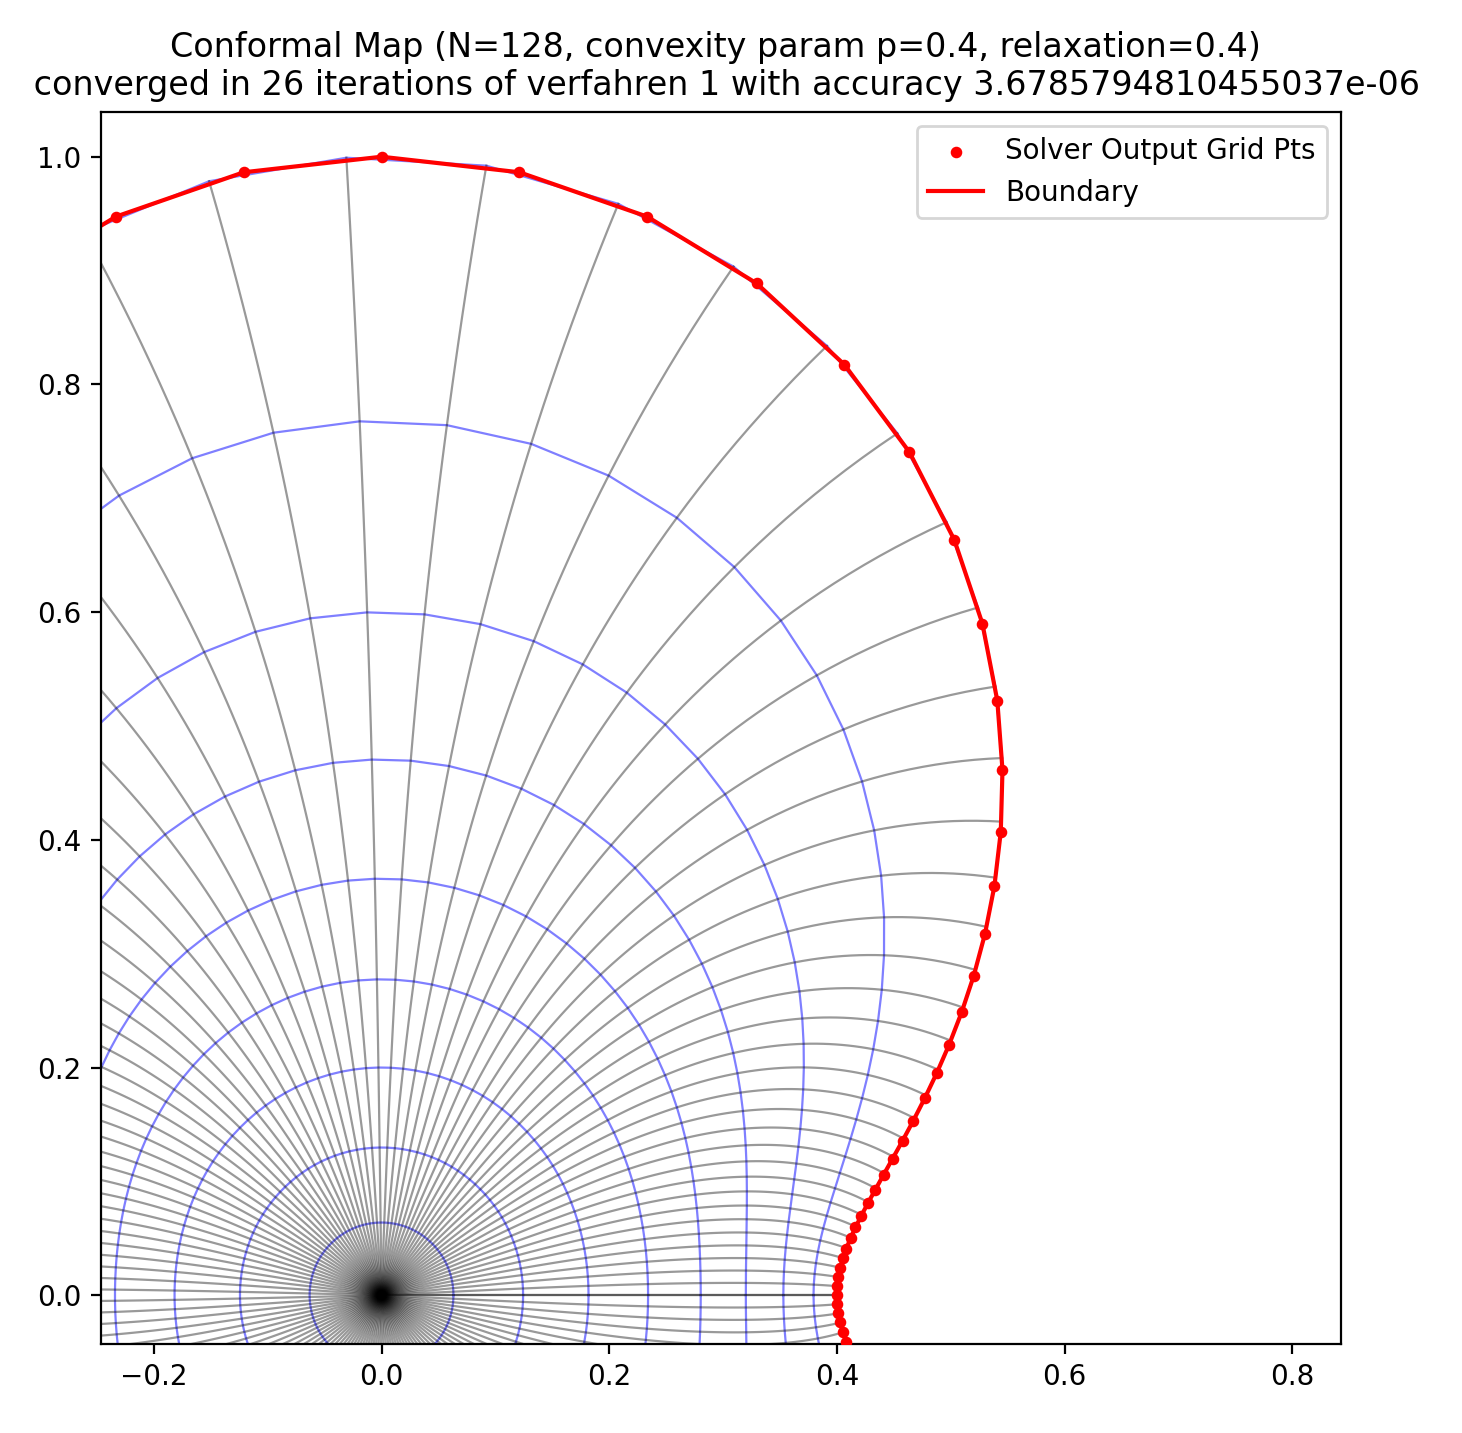
\includegraphics[width=0.5\textwidth]{img/invellip_v1_p4_r4_detail.png}
    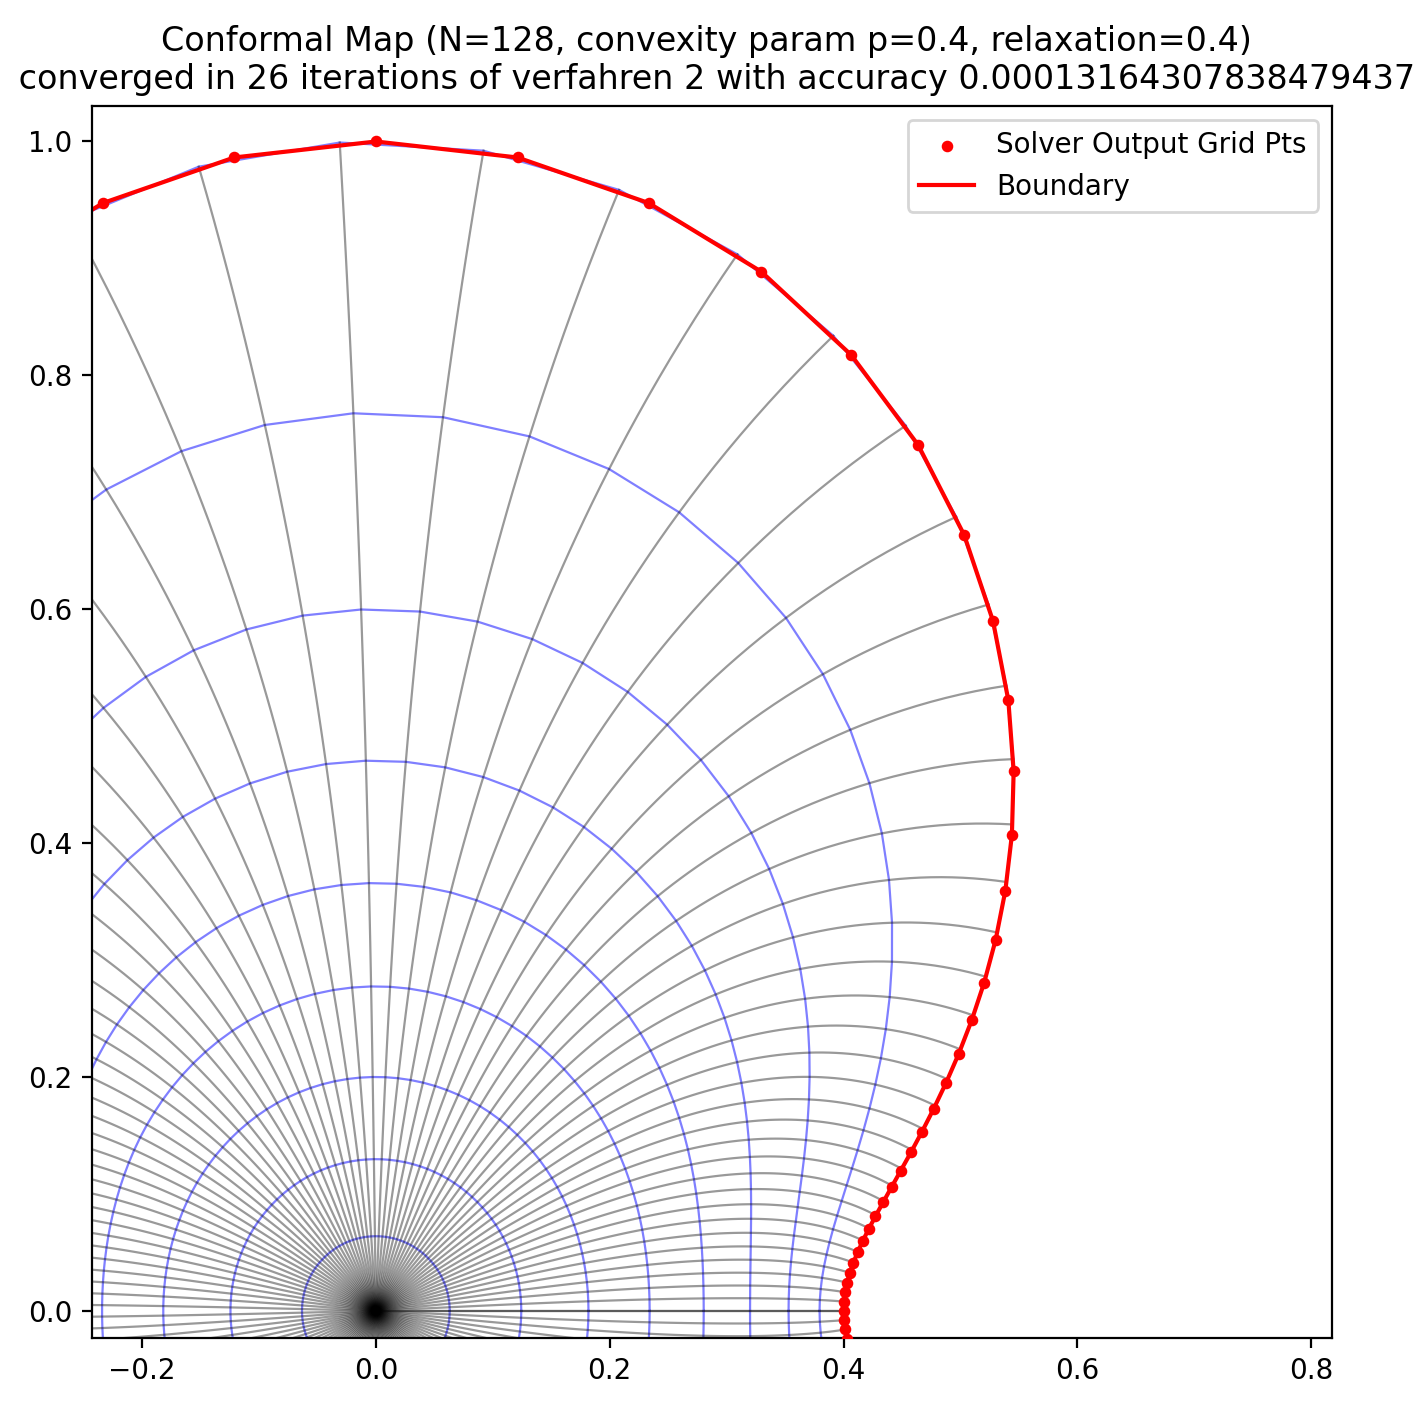
\includegraphics[width=0.5\textwidth]{img/invellip_v2_p4_r4_detail.png}
    \caption{Gaier's inverted ellipse with convexity parameter $p = 0.4$.\\ 
    \cite[Anhang 5]{Gaier1964}}
\end{figure}
\begin{table}[H]
    \centering
    \caption{Inverted ellipse discretized at $N = 512$ points, with convexity parameter $p = 0.4$.}
    \begin{tabular}{|p{0.2\textwidth}|p{0.35\textwidth}|p{0.35\textwidth}|}
        \hline
        Verfahren & 1 & 2 \\
        \hline
        Accuracy & 1.5891462382292706e-06 & 1.5891462375908835e-06 \\
        \hline
        Iteration \# & \multicolumn{2}{c|}{Norm of correction/ update step $\lVert U_{k} \rVert$} \\
        0 & 146.31078308548652 & 146.31078308548652 \\
        1 & 95.99285028612374 & 95.99285028612373 \\
        2 & 61.15293523092539 & 61.15293523092546 \\
        3 & 38.121296929641325 & 38.12129692964127 \\
        4 & 23.41997703097582 & 23.41997703097586 \\
        5 & 14.255599037451171 & 14.255599037451175 \\
        6 & 8.627969413050884 & 8.627969413050833 \\
        7 & 5.203900815255897 & 5.203900815255858 \\
        8 & 3.1321557040508266 & 3.132155704050878 \\
        9 & 1.882837647726864 & 1.8828376477268935 \\
        10 & 1.13098075422205 & 1.130980754222054 \\
        \dots & \dots & \dots \\
        29 & 6.903442316958354e-05 & 6.90344231315847e-05 \\
        \hline
    \end{tabular}
\end{table}

\newpage
%%%%%%%%%%%%%%%%%%% INVERTED ELLIPSE p = 0.3 %%%%%%%%%%%%%%%%%%%
We have tried making this example even more convex, but already $p=0.3$ is quite a challenge, relaxation must be chosen extremely small and thus convergence takes much longer.
\begin{figure}[H]
    \caption{Accuracy of conformal map on inverted ellipse, $p = 0.3$: \\
    Verfahren 1: $3.710212908531002e-06$, Verfahren 2: $3.7636081451245516e-06$}
    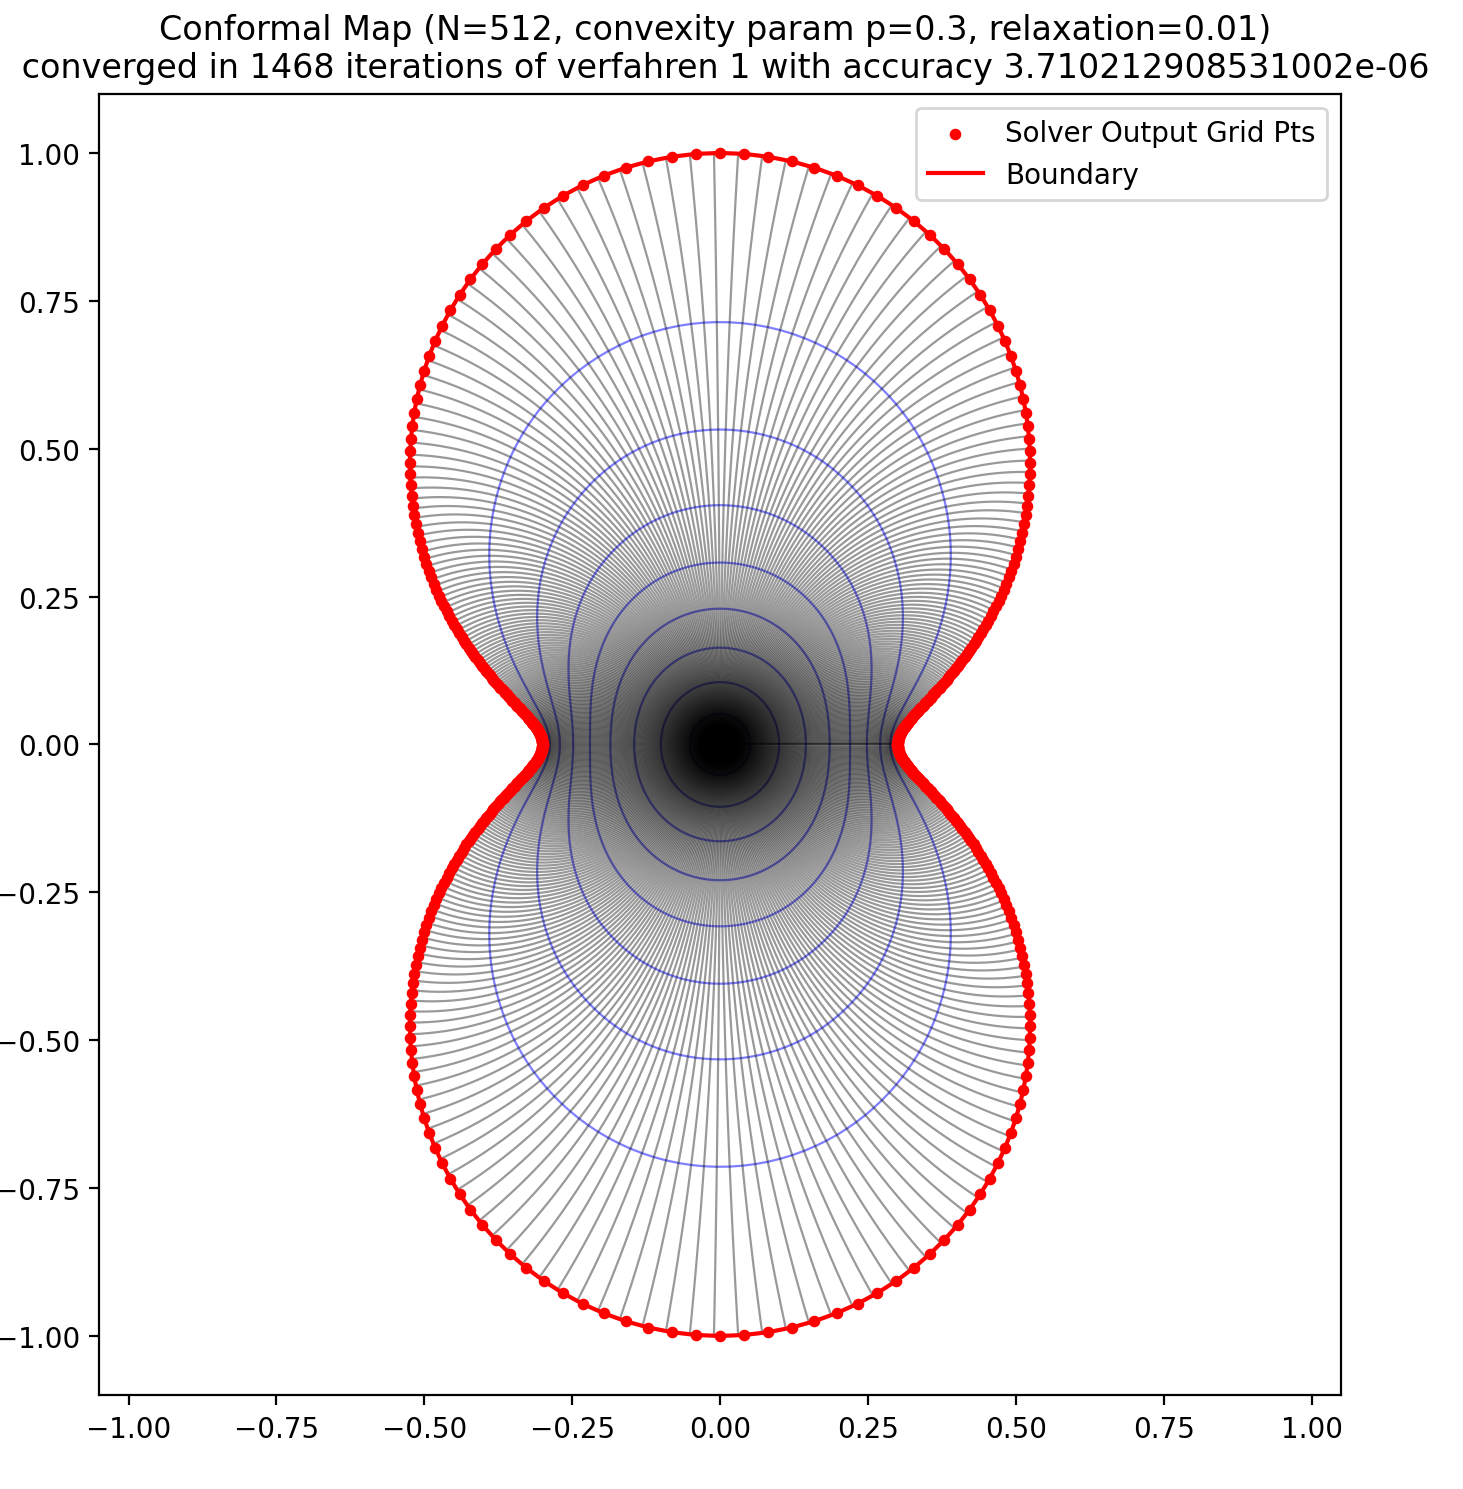
\includegraphics[width=0.5\textwidth]{img/invellip_v1_p3.png}
    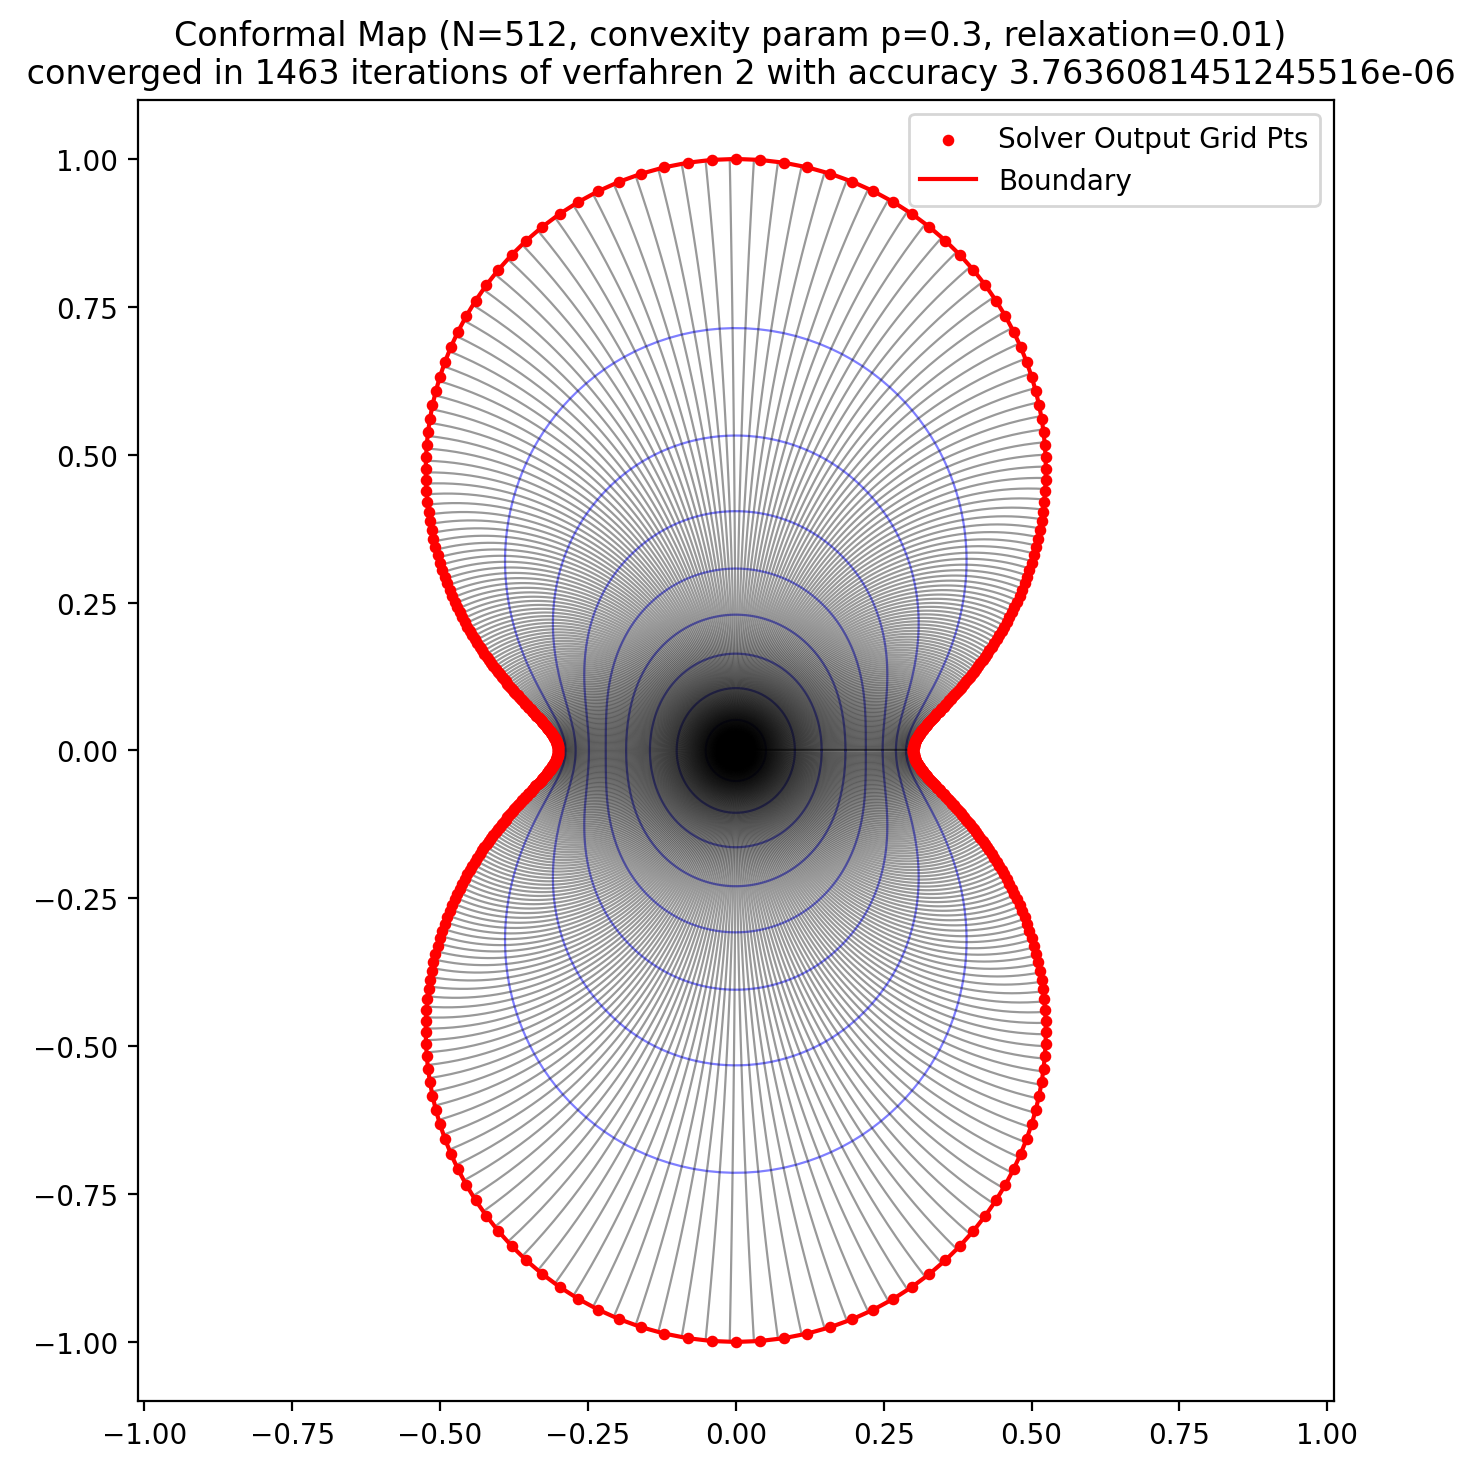
\includegraphics[width=0.5\textwidth]{img/invellip_v2_p3.png}
    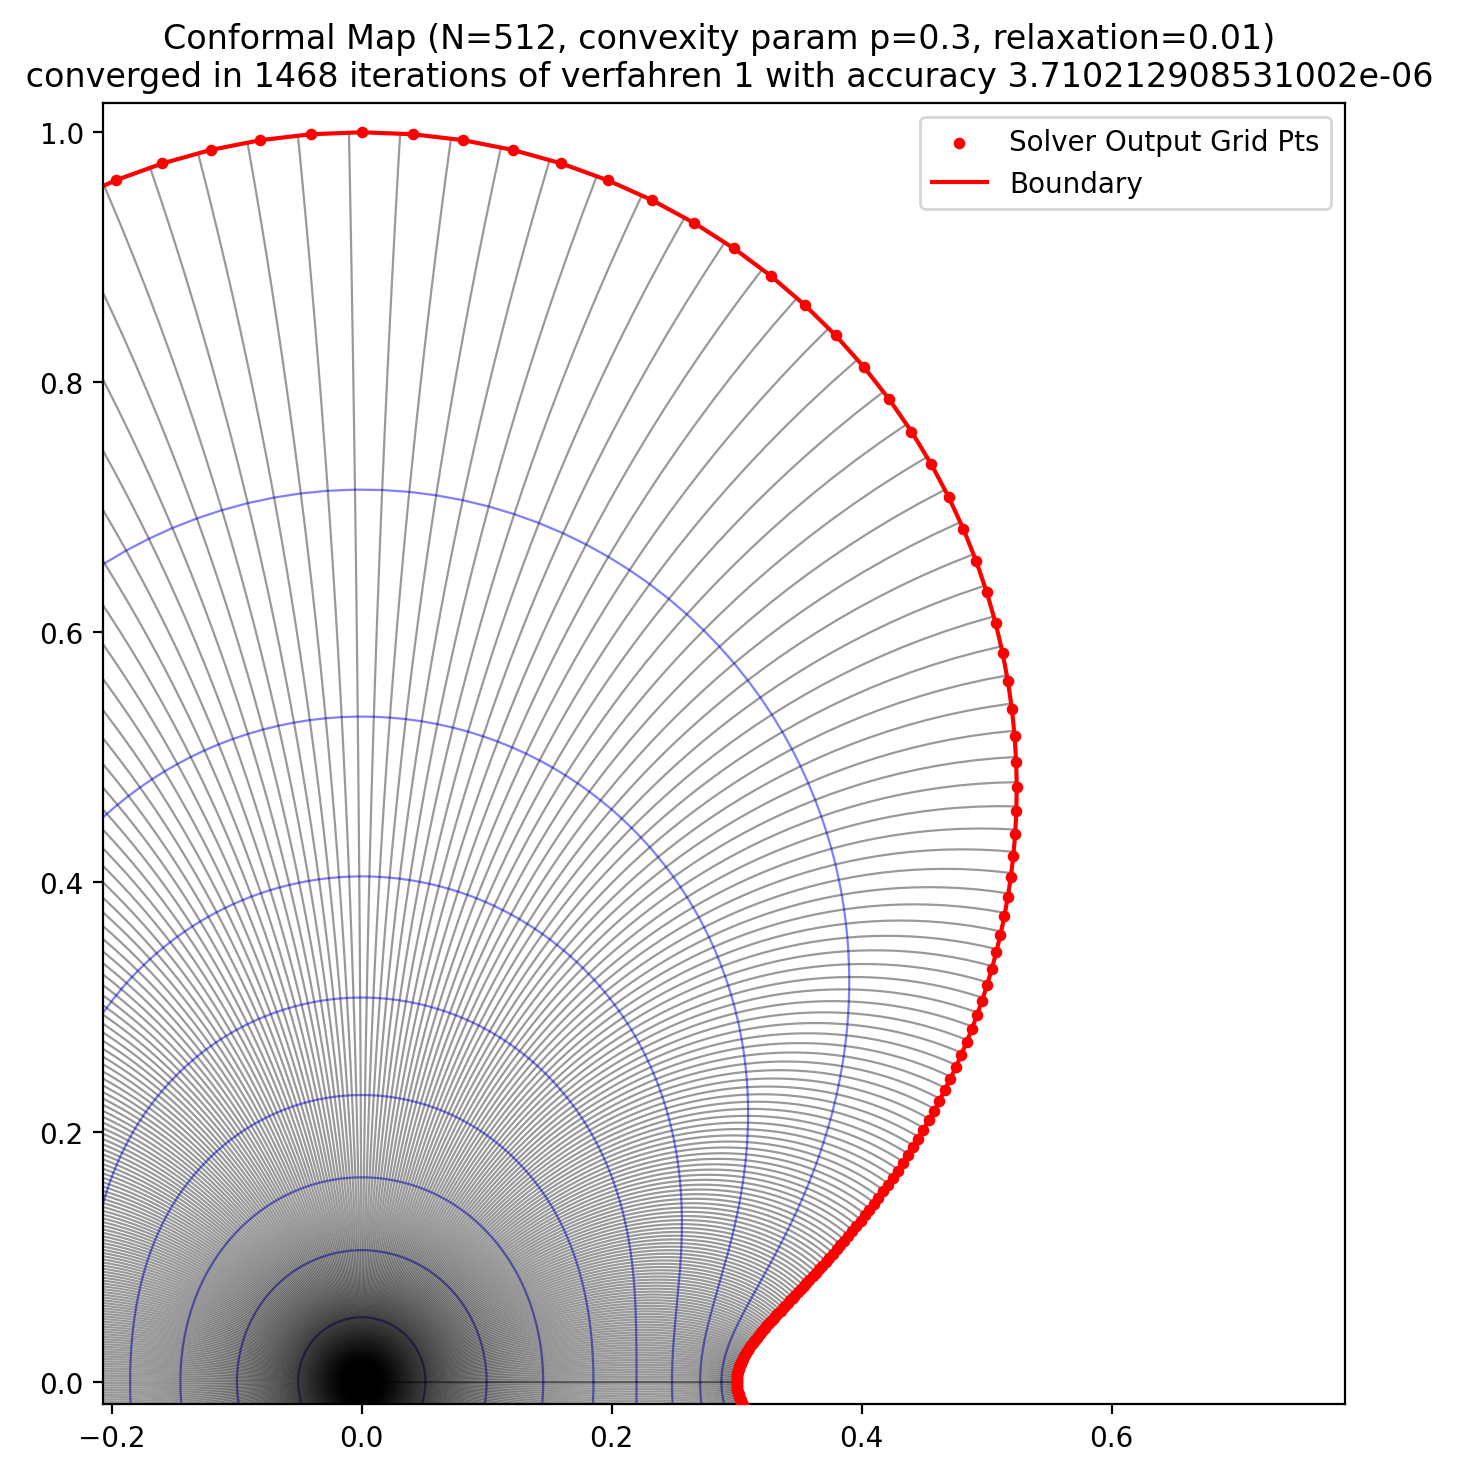
\includegraphics[width=0.5\textwidth]{img/invellip_v1_p3_detail.png}
    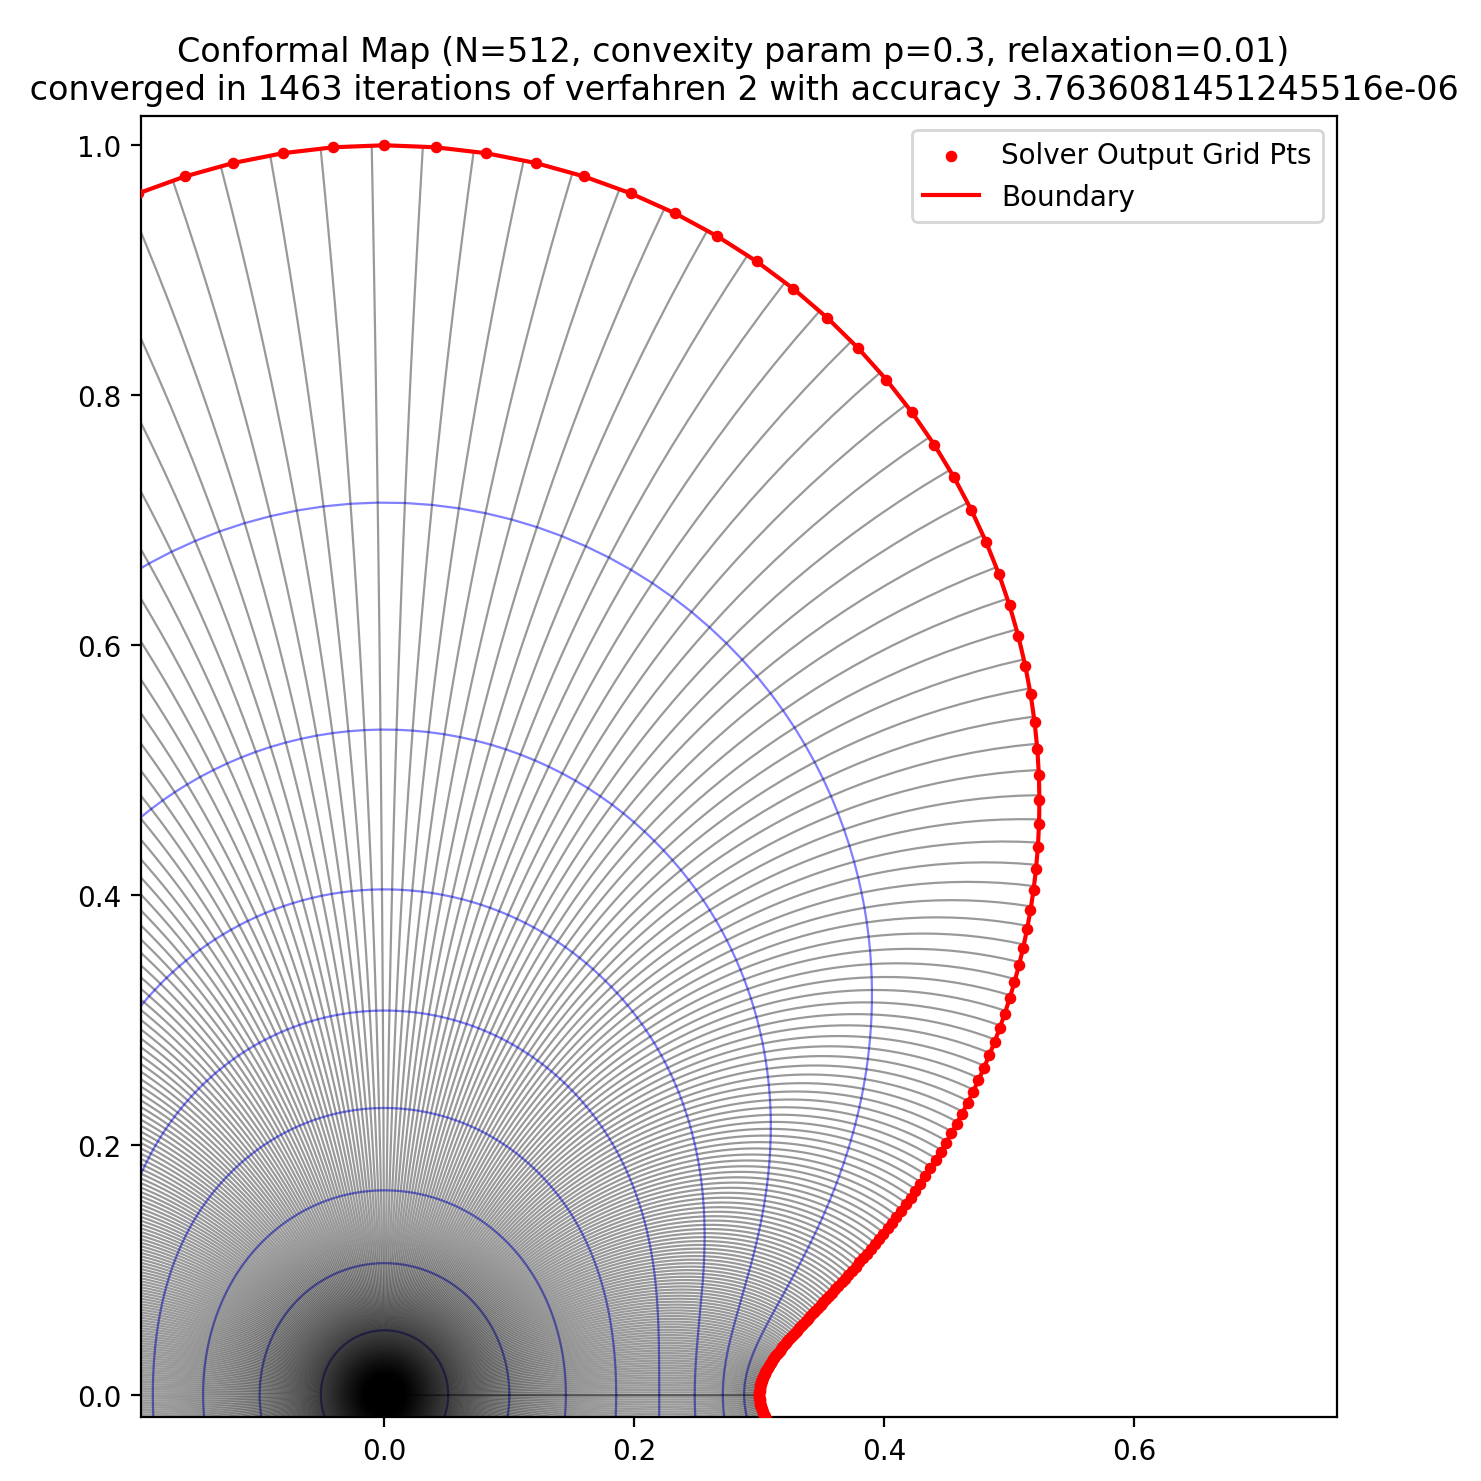
\includegraphics[width=0.5\textwidth]{img/invellip_v2_p3_detail.png}
\end{figure}
\iffalse
%%%%%%%%%%%% SOMETHING %%%%%%%%%%%%%%%%%%%
\begin{figure}[H]
    %\includegraphics[width=0.5\textwidth]{}
    %\includegraphics[width=0.5\textwidth]{}
    \caption{AAAAAAAAAAAAAAAA}
\end{figure}
\begin{table}[H]\centering
    \caption{AAAAAAAAAAAAAAAAAAAA.}
    \centering
    \begin{tabular}{|p{0.2\textwidth}|p{0.35\textwidth}|p{0.35\textwidth}|}
        \hline
        Verfahren & 1 & 2 \\
        \hline
        Accuracy &  &  \\
        \hline
        Iteration \# & \multicolumn{2}{c}{Norm of correction/ update step $\lVert U_{k} \rVert$} \\
        0 &  &  \\
        1 &  &  \\
        2 &  &  \\
        3 &  &  \\
        4 &  &  \\
        5 &  &  \\
        6 &  &  \\
        7 &  &  \\
        8 &  &  \\
        9 &  &  \\
        10 &  &  \\
        \dots & \dots & \dots \\
        75 &  &  \\
        \dots & \dots &  \\
        150 &  &  \\

        \hline
    \end{tabular}
\end{table}

%%%%%%%%%%%% WHATEVER (ADD FLOWER WHERE ONE CONVERGES AND ONE DOESNT)%%%%%%%%%%%%%%%%%%%
\begin{figure}[H]\centering
    %\includegraphics[width=0.5\textwidth]{}
    %\includegraphics[width=0.5\textwidth]{}
    \caption{AAAAAAAAAAAAAAAA}
\end{figure}
\begin{table}[H]\centering
    \caption{aaaaaaaaaaaaaaaaaaaaa.}
    \centering
    \begin{tabular}{|p{0.2\textwidth}|p{0.35\textwidth}|p{0.35\textwidth}|}
        \hline
        Verfahren & 1 & 2 \\
        \hline
        Accuracy &  &  \\
        \hline
        Iteration \# & \multicolumn{2}{c}{Norm of correction/ update step $\lVert U_{k} \rVert$} \\
        0 &  &  \\
        1 &  &  \\
        2 &  &  \\
        3 &  &  \\
        4 &  &  \\
        5 &  &  \\
        6 &  &  \\
        7 &  &  \\
        8 &  &  \\
        9 &  &  \\
        10 &  &  \\
        \dots & \dots & \dots \\
        75 &  &  \\
        \dots & \dots &  \\
        150 &  &  \\

        \hline
    \end{tabular}
\end{table}
\fi

\red{Note for example the flower with 8 petals on the front page of this paper. When choosing convexity parameter as high as $p=0.5$, Wegmann's solver converges only using the second Verfahren. WHY?}

\begin{figure}[H]
    \caption{Truncated Square}
    \label{fig:truncatedSquare}
    \centering
    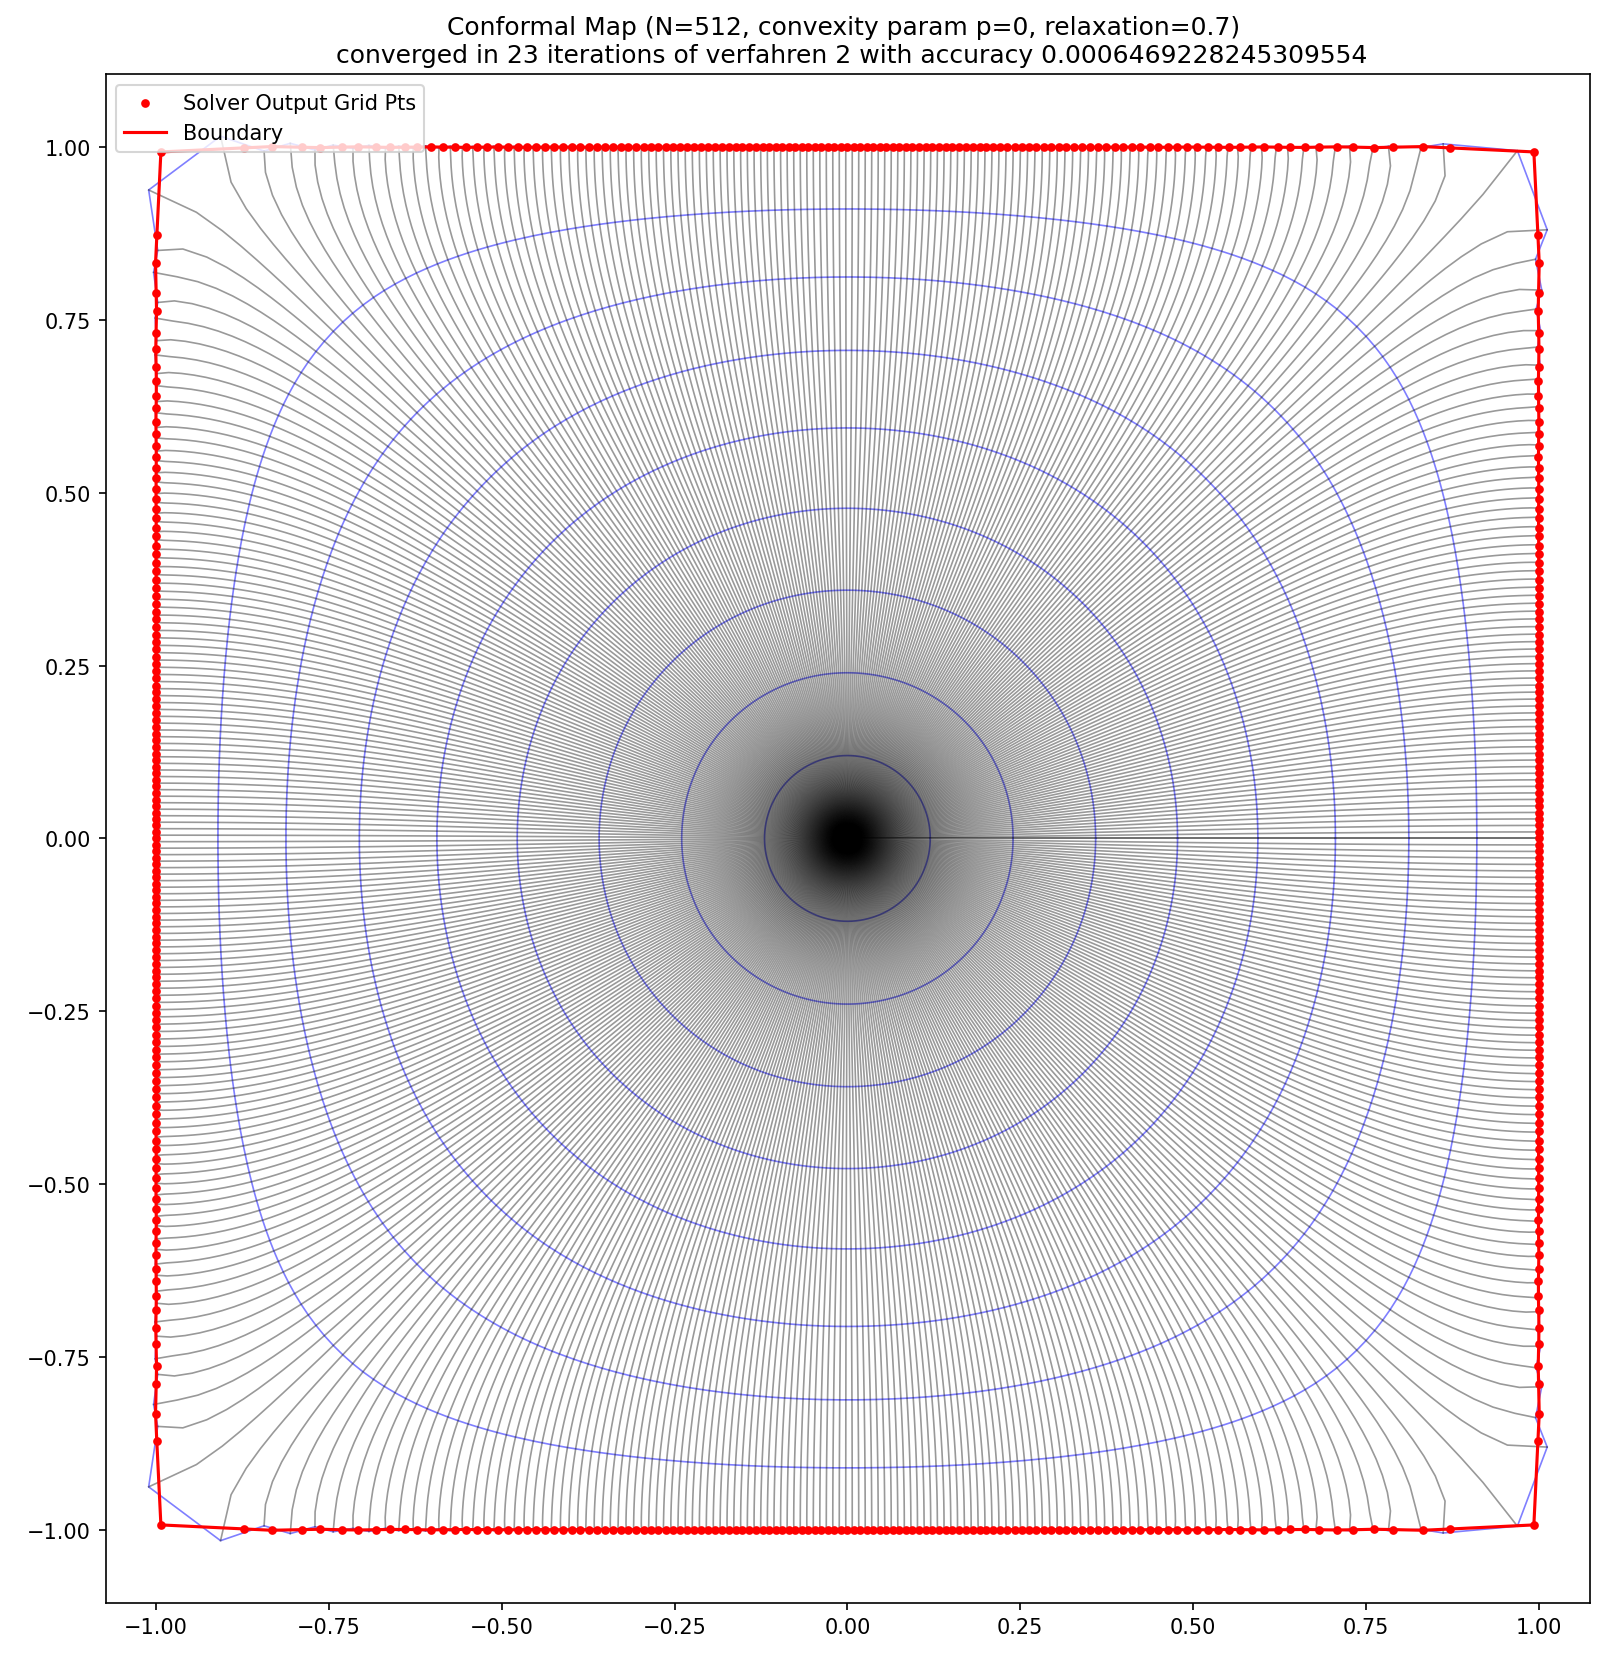
\includegraphics[height=0.5\textheight]{img/square.png}%
    \vfill
    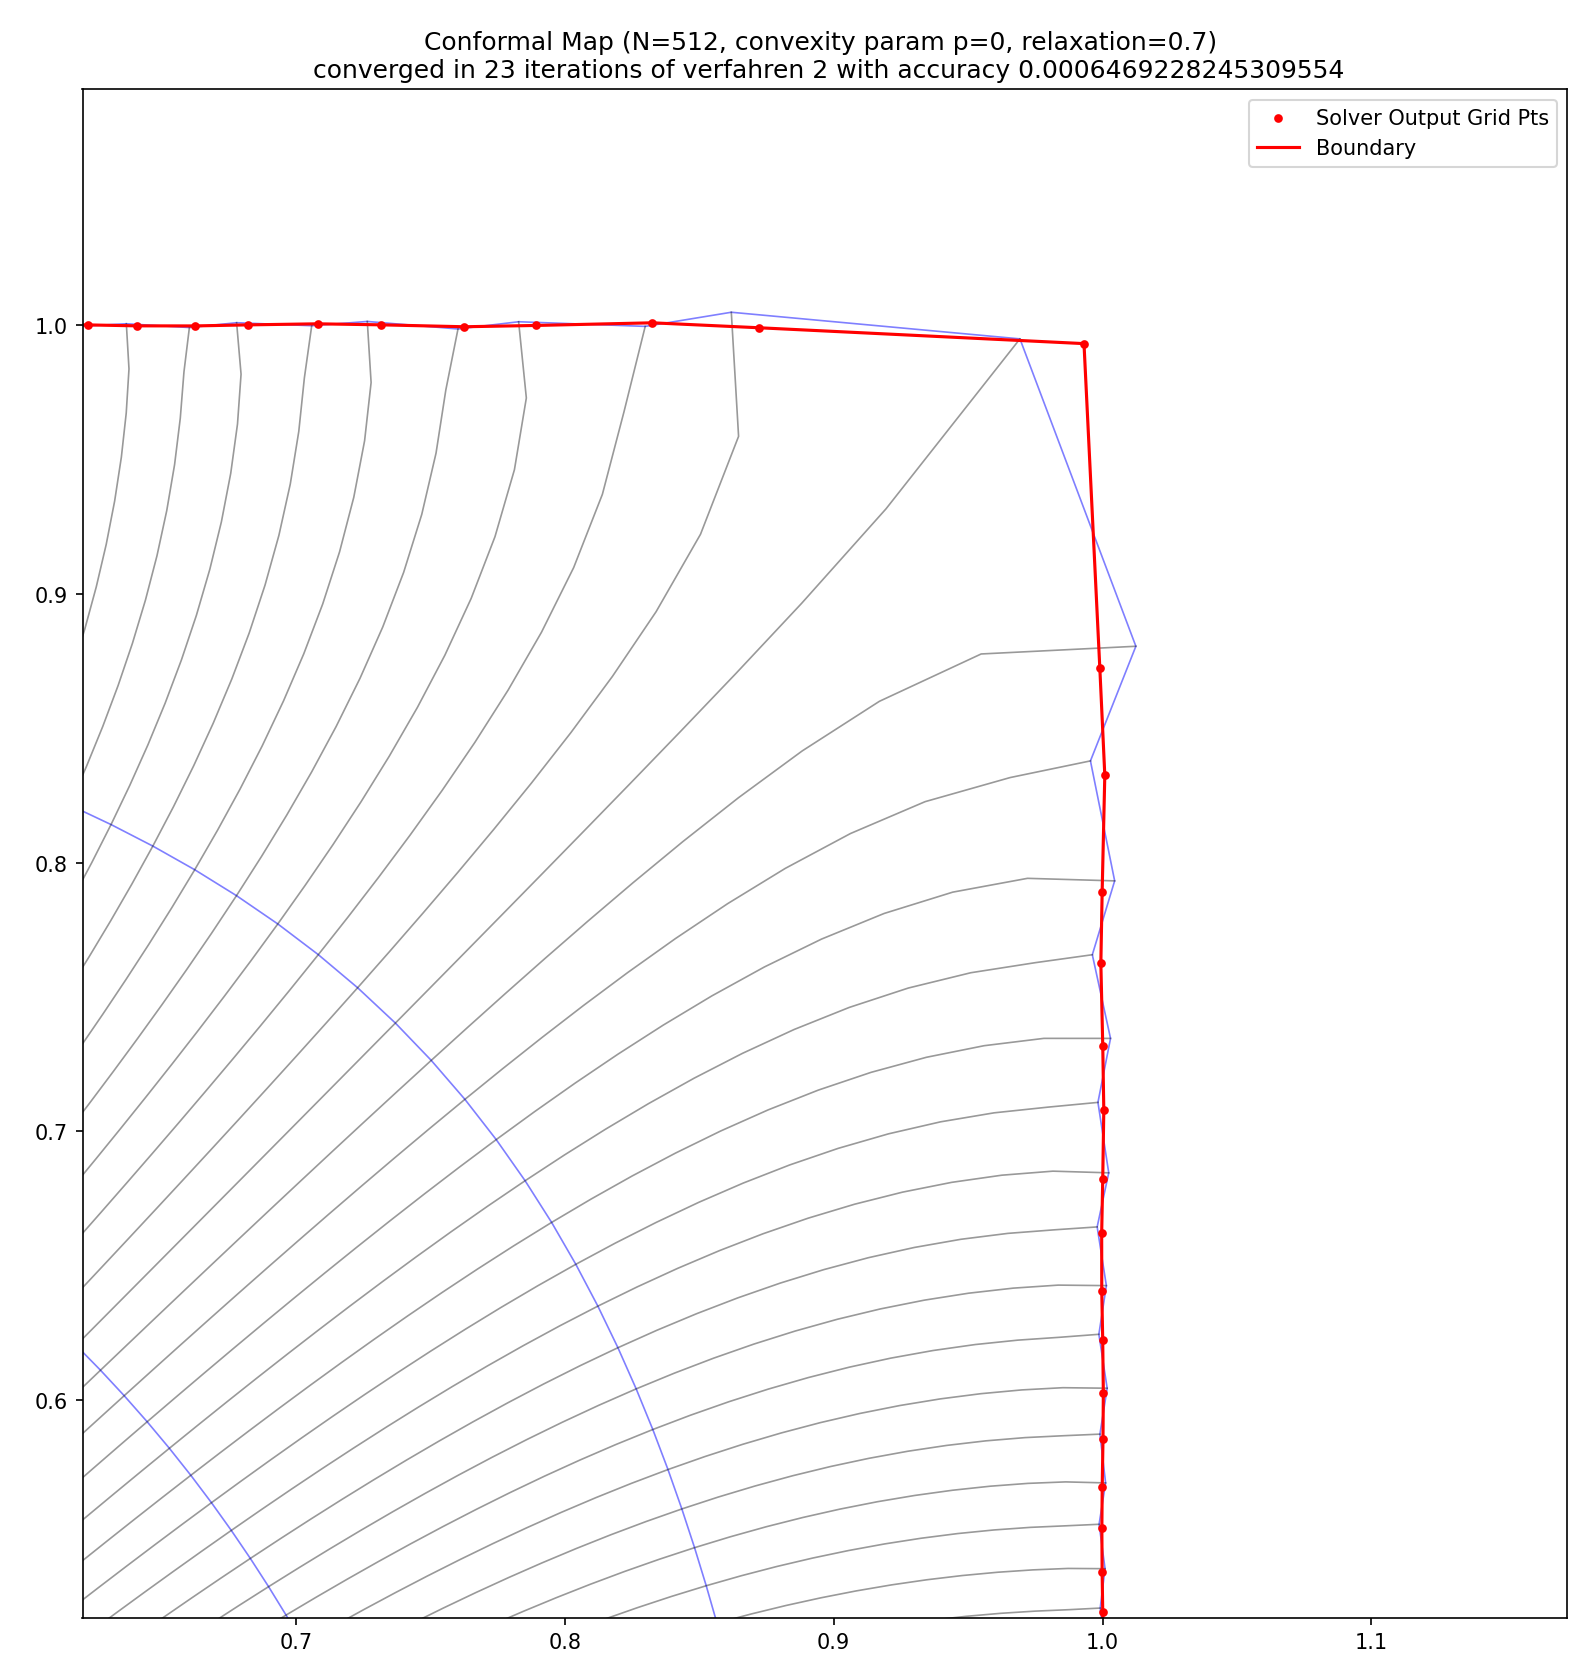
\includegraphics[height=0.5\textheight]{img/square_detail.png}
\end{figure}
It also it worth noting that for the example of the truncated square, only method 2 converges with a usable accuracy and relaxation. Method 1 diverges after the 1500th iteration even when choosing a relaxation factor as low as 1e-3. Verfahren 2 in turn converges incredibly quickly even with relaxation of only 0.7, as depicted in Figure \ref{fig:truncatedSquare}.


\begin{figure}[H]\centering
    \caption{A good initial guess is vital, as the algorithm is only guaranteed to converge locally quadratically for a close enough initial guess. The result of trying to find the map onto a kite by choosing the unit disk as initial guess is shown here.}
    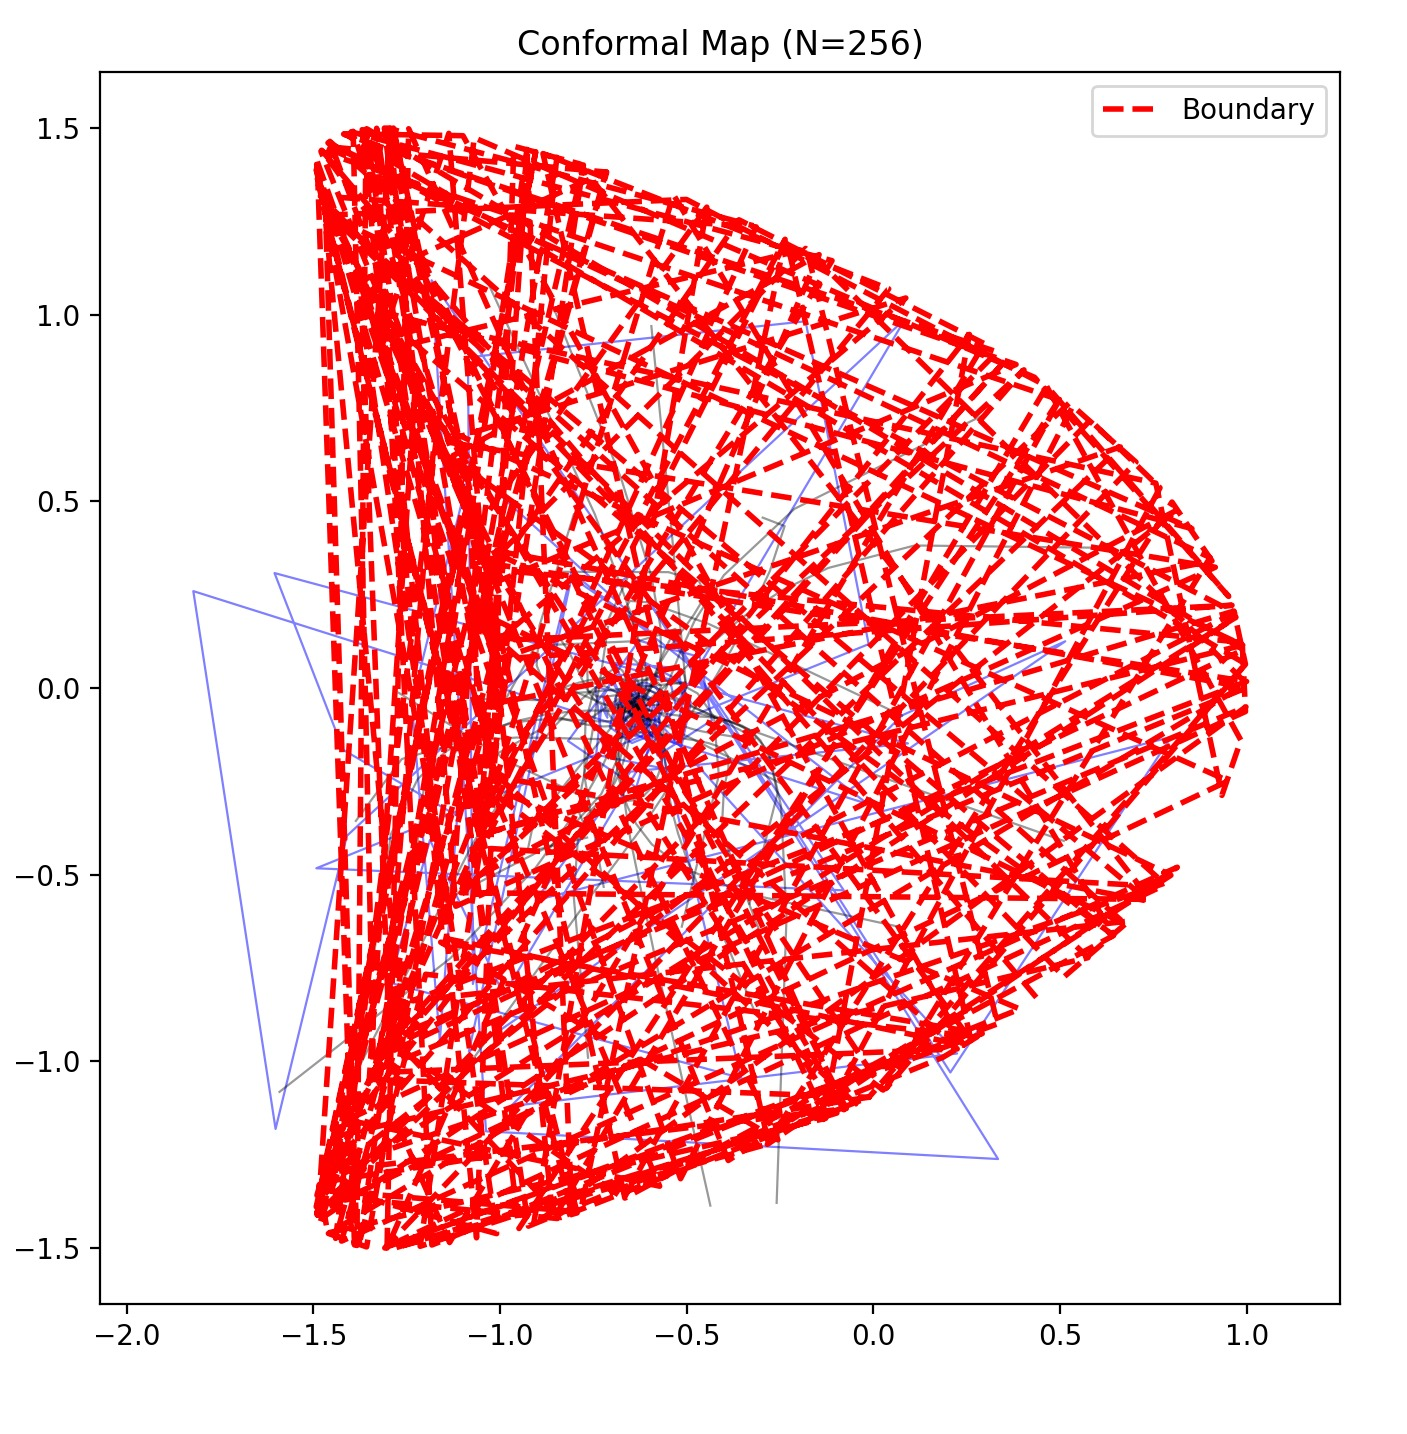
\includegraphics[width=0.6\textwidth]{kite_initial_guess_circle.jpeg}
\end{figure}
\begin{figure}[H]\centering
    \caption{In this case, the initial guess was chosen to be a star, which shares some of the properties with the kite's tangent vector, but it is still too convex and therefore far away from the kite to guarantee convergence of the solver.}
    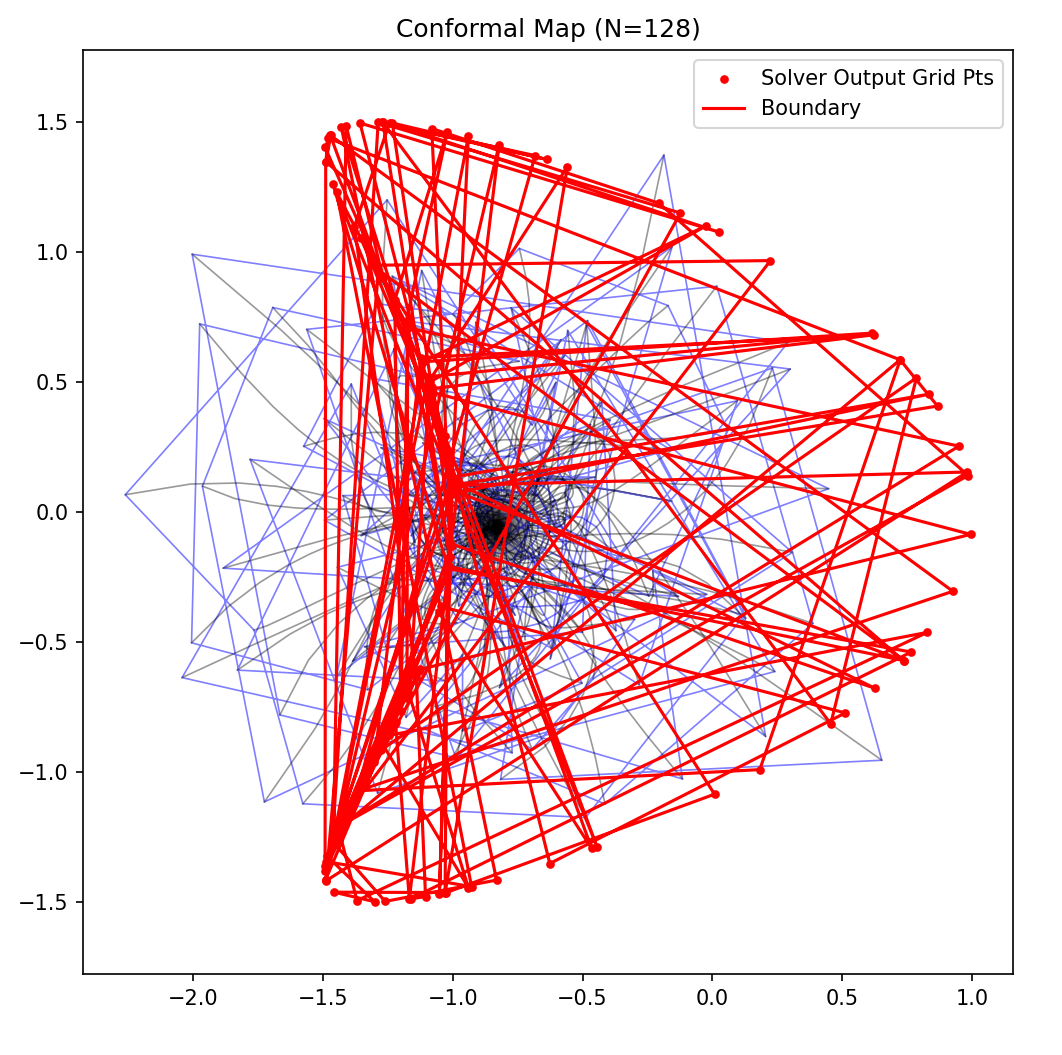
\includegraphics[width=0.6\textwidth]{kite_divergence_gibbs.png}
\end{figure}
The solver has proven experimentally not to converge on the kite region parametrised by     
\begin{equation}
    k(s) = (\text{cos}(s) + 0.65\text{cos}(2s) - 0.65, 1.5 \text{sin}(s)) \text{ for }s \in [0,2\pi].
\end{equation}
A homotopy algorithm is a possible solution to this, which we omit due to time constraints. The idea is as follows: the parameter 0.65 is relaxed and a sequence of intermediate regions is computed, where each solution is the initial guess for the subsequent mapping.
